\documentclass[runningheads]{llncs}

% multiple footnotes
%\usepackage[para]{footmisc}

\usepackage{bold-extra}
\usepackage[scaled]{helvet}

% graphics
\usepackage{adjustbox}
\usepackage{stfloats}
\usepackage{graphicx}
\usepackage[dvipsnames]{xcolor}
\usepackage{xspace}
\usepackage{stmaryrd}
\usepackage{wrapfig}
\usepackage{textcomp}
\usepackage[textsize=footnotesize]{todonotes}
\usepackage{quantikz}
\usepackage{amsmath}
\newenvironment{smallmat}{\left[\begin{smallmatrix}}{\end{smallmatrix}\right]}

\newenvironment{compactwrapfigure}
     {\setlength{\columnsep}{0pt}
      \wrapfloat{figure}}
     {\endwrapfloat}

\usepackage{caption}
\usepackage{subcaption}

\usepackage{stmaryrd}
\usepackage{paralist}
\usepackage{mathtools}
\usepackage{braket}

% orcid logo with hyperlinks enabled
\newcommand\UrlFont{\color{blue}\rmfamily}
\makeatletter
\RequirePackage[bookmarks,unicode,colorlinks=true]{hyperref}%
\def\@citecolor{blue}%
\def\@urlcolor{blue}%
\def\@linkcolor{blue}%
\def\UrlFont{\rmfamily}
\def\orcid#1{\,\smash{\href{http://orcid.org/#1}{\protect\raisebox{1pt}{\protect\includegraphics{orcid_color.eps}}}}}
\makeatother

\usepackage{hyperref}
%\usepackage[title]{appendix}

% tables
\usepackage{tabularx}
\usepackage{rotating}
\usepackage{multirow}
\usepackage{tablefootnote}
\usepackage{cite}
\usepackage{siunitx}
\usepackage{colortbl}

% long equations
\usepackage{amsmath,amssymb, bm}
\usepackage{dsfont}
\usepackage{paralist}

% special symbols
\usepackage{pifont}

\newcommand{\xmark}{\ding{55}}

% define titlesec properly with llncs
\let\llncssubparagraph\subparagraph
\let\subparagraph\paragraph
\usepackage{titlesec}
\let\subparagraph\llncssubparagraph
%\titleformat{\paragraph}[runin]
%{\bfseries\itshape}{\theparagraph}{}{}

% for letter symbol
\usepackage[misc,geometry]{ifsym} 

%define a marking command
\newcommand{\HiLi}[2]{\leavevmode\rlap{\hbox to \hsize{\color{#1!#2}\leaders\hrule height .7\baselineskip depth .75ex\hfill}}}

% algorithms
\usepackage[ruled,linesnumbered,noline,noend]{algorithm2e}
\usepackage{algpseudocode, setspace}
\usepackage{tcolorbox}
\newcommand\mycommfont[1]{\ttfamily\textcolor{OliveGreen}{#1}}

% parallel for-loop
\SetKwFor{ForAllPar}{forall}{do in parallel}{endfor}
\SetKwFor{Forparx}{for all ${\normalfont \tidx} \in \llbracket$}{$\rrbracket^\td{x}$ do in parallel}{end}
\SetKwFor{Forpary}{for all ${\normalfont \tidy}\in \llbracket$}{$\rrbracket^\td{y}$ do in parallel}{end}

% Definition of kernel function
\SetKwProg{Kernel}{\textit{device kernel}}{:}{}
\SetKwProg{Devfunction}{\textit{device function}}{:}{}
\SetKwProg{Function}{\textit{function}}{:}{}

% Tikz config.
\usepackage{tikz}
\usetikzlibrary{fit,calc}

\let\oldnl\nl% Store \nl in \oldnl
\newcommand{\nonl}{\renewcommand{\nl}{\let\nl\oldnl}}% Remove line number for one line
%

% align line numbers in algorithms
\usepackage{etoolbox}
\makeatletter
\patchcmd\algocf@Vline{\vrule}{\vrule \kern-0.4pt}{}{}
\patchcmd\algocf@Vsline{\vrule}{\vrule \kern-0.4pt}{}{}
\makeatother

%\setlength{\parskip}{0pt}
\setlength{\textfloatsep}{10pt}

% All notations should be defined here
% to avoid going up and down .

% format pseudcode
\newcommand{\code}[1]{{{\texttt{#1}}}}
\newcommand{\var}[1]{\texttt{#1}}
\newcommand{\routine}[1]{{\relsize{0.5}{\textsc{#1}}}}
\newcommand{\tool}[1]{{\relsize{-0.4}{\textsc{#1}}}}
\newcommand{\return}{\textbf{return}\xspace}
\newcommand{\Break}{\textbf{break}\xspace}
\newcommand{\true}{\textbf{true}\xspace}
\newcommand{\false}{\textbf{false}\xspace}
\newcommand{\fast}[1]{\textcolor{Green}{\ensuremath{\blacktriangle}} #1}
\newcommand{\slow}[1]{\textcolor{Red}{\ensuremath{\blacktriangledown}} #1}
\newcommand{\td}[1]{\textbf{\var{#1}}\xspace}
\newcommand{\li}[1]{l.\ref{#1}}
\newcommand{\lis}[2]{l.\ref{#1}-\ref{#2}}
\colorlet{gpu}{violet}

% Notations
\newcommand{\numQubits}{\ensuremath{n}\xspace}
\newcommand{\depth}{\ensuremath{d}\xspace}
\newcommand{\clifford}{\ensuremath{\mathcal{C}}\xspace}
\newcommand{\cliffordGroup}{\ensuremath{\mathcal{G}}\xspace}
\newcommand{\tableau}{\ensuremath{\mathcal{T}}\xspace}
\newcommand{\partition}{\ensuremath{p}\xspace}
\newcommand{\tableauPartition}{\tableau\xspace}
\newcommand{\tableauWidth}{\numQubits\xspace}
\newcommand{\tableauHeight}{\ensuremath{k}\xspace}
\newcommand{\dep}{\ensuremath{\mathcal{D}}\xspace}
\newcommand{\newGate}{\ensuremath{g}\xspace}
\newcommand{\circuitQueue}{\clifford\xspace}
\newcommand{\circuitWindow}{\ensuremath{\mathcal{W}}\xspace}
\newcommand{\circuitScheduled}{\ensuremath{\mathcal{P}}\xspace}
\newcommand{\lockedSet}{\ensuremath{L}\xspace}
\newcommand{\wires}{\ensuremath{\mathcal{Q}}\xspace}
\newcommand{\qubit}{\ensuremath{q}\xspace}
\newcommand{\tx}{\ensuremath{\var{t}_{\td{x}}}\xspace}
\newcommand{\ty}{\ensuremath{\var{t}_{\td{y}}}\xspace}
\newcommand{\blockDim}{\var{xBlockSize}\xspace}
\newcommand{\stride}{\var{stride}\xspace}
\newcommand{\tid}{\var{tid}\xspace}
\newcommand{\tidy}{\ensuremath{\tid_{\td{y}}}\xspace}
\newcommand{\tidx}{\ensuremath{\tid_{\td{x}}}\xspace}

% Algorithmic notations
\newcommand{\pickFront}{\routine{pickFrontGate}\xspace}
\newcommand{\initTableau}{\routine{createInitialState}\xspace}
\newcommand{\simulateWindow}{\routine{simulateWindow}\xspace}
\newcommand{\copyToDevice}{\routine{copyToDeviceAsync}\xspace}
\newcommand{\sync}{\routine{synchronizeDevice}\xspace}
\newcommand{\allocate}{\routine{allocateTableau}\xspace}
\newcommand{\Swap}{\routine{swap}\xspace}
\newcommand{\syncThreads}{\routine{synchronizeThreads}\xspace}
\newcommand{\atomicXOR}{\routine{atomicXOR}\xspace}
\newcommand{\collapseSigns}{\routine{collapseSigns}\xspace}
\newcommand{\numPartitions}{\var{numPartitions}\xspace}
\newcommand{\partitionSize}{\var{tableauSize}\xspace}
\newcommand{\partitionOffset}{\var{tableauOffset}\xspace}
\newcommand{\copyStream}{\var{copyStream}\xspace}
\newcommand{\kernelStream}{\var{kernelStream}\xspace}
\newcommand{\generator}{\var{generator}\xspace}
\newcommand{\gateWires}{\var{gateWires}\xspace}
\newcommand{\parGate}{\var{parallelGate}\xspace}
\newcommand{\sign}{\var{s}\xspace}
\newcommand{\shared}{\var{shared}\xspace}
\newcommand{\maxThreads}{\ensuremath{T}\xspace}

% tools
\newcommand{\stim}{\tool{Stim}\xspace}
\newcommand{\qiskit}{\tool{Qiskit}\xspace}
\newcommand{\quasarq}{\tool{QuaSARQ}\xspace}


% Proof trees
\message{<Paul Taylor's Proof Trees, 2 August 1996>}
%% Build proof tree for Natural Deduction, Sequent Calculus, etc.
%% WITH SHORTENING OF PROOF RULES!
%% Paul Taylor, begun 10 Oct 1989
%% *** THIS IS ONLY A PRELIMINARY VERSION AND THINGS MAY CHANGE! ***
%%
%% 2 Aug 1996: fixed \mscount and \proofdotnumber
%%
%%      \prooftree
%%              hyp1            produces:
%%              hyp2
%%              hyp3            hyp1    hyp2    hyp3
%%      \justifies              -------------------- rulename
%%              concl                   concl
%%      \thickness=0.08em
%%      \shiftright 2em
%%      \using
%%              rulename
%%      \endprooftree
%%
%% where the hypotheses may be similar structures or just formulae.
%%
%% To get a vertical string of dots instead of the proof rule, do
%%
%%      \prooftree                      which produces:
%%              [hyp]
%%      \using                                  [hyp]
%%              name                              .
%%      \proofdotseparation=1.2ex                 .name
%%      \proofdotnumber=4                         .
%%      \leadsto                                  .
%%              concl                           concl
%%      \endprooftree
%%
%% Within a prooftree, \[ and \] may be used instead of \prooftree and
%% \endprooftree; this is not permitted at the outer level because it
%% conflicts with LaTeX. Also,
%%      \Justifies
%% produces a double line. In LaTeX you can use \begin{prooftree} and
%% \end{prootree} at the outer level (however this will not work for the inner
%% levels, but in any case why would you want to be so verbose?).
%%
%% All of of the keywords except \prooftree and \endprooftree are optional
%% and may appear in any order. They may also be combined in \newcommand's
%% eg "\def\Cut{\using\sf cut\thickness.08em\justifies}" with the abbreviation
%% "\prooftree hyp1 hyp2 \Cut \concl \endprooftree". This is recommended and
%% some standard abbreviations will be found at the end of this file.
%%
%% \thickness specifies the breadth of the rule in any units, although
%% font-relative units such as "ex" or "em" are preferable.
%% It may optionally be followed by "=".
%% \proofrulebreadth=.08em or \setlength\proofrulebreadth{.08em} may also be
%% used either in place of \thickness or globally; the default is 0.04em.
%% \proofdotseparation and \proofdotnumber control the size of the
%% string of dots
%%
%% If proof trees and formulae are mixed, some explicit spacing is needed,
%% but don't put anything to the left of the left-most (or the right of
%% the right-most) hypothesis, or put it in braces, because this will cause
%% the indentation to be lost.
%%
%% By default the conclusion is centered wrt the left-most and right-most
%% immediate hypotheses (not their proofs); \shiftright or \shiftleft moves
%% it relative to this position. (Not sure about this specification or how
%% it should affect spreading of proof tree.)
%
% global assignments to dimensions seem to have the effect of stretching
% diagrams horizontally.
%
%%==========================================================================

\def\introrule{{\cal I}}\def\elimrule{{\cal E}}%%
\def\andintro{\using{\land}\introrule\justifies}%%
\def\impelim{\using{\Rightarrow}\elimrule\justifies}%%
\def\allintro{\using{\forall}\introrule\justifies}%%
\def\allelim{\using{\forall}\elimrule\justifies}%%
\def\falseelim{\using{\bot}\elimrule\justifies}%%
\def\existsintro{\using{\exists}\introrule\justifies}%%

%% #1 is meant to be 1 or 2 for the first or second formula
\def\andelim#1{\using{\land}#1\elimrule\justifies}%%
\def\orintro#1{\using{\lor}#1\introrule\justifies}%%

%% #1 is meant to be a label corresponding to the discharged hypothesis/es
\def\impintro#1{\using{\Rightarrow}\introrule_{#1}\justifies}%%
\def\orelim#1{\using{\lor}\elimrule_{#1}\justifies}%%
\def\existselim#1{\using{\exists}\elimrule_{#1}\justifies}

%%==========================================================================

\newdimen\proofrulebreadth \proofrulebreadth=.05em
\newdimen\proofdotseparation \proofdotseparation=1.25ex
\newdimen\proofrulebaseline \proofrulebaseline=2ex
\newcount\proofdotnumber \proofdotnumber=3
\let\then\relax
\def\hfi{\hskip0pt plus.0001fil}
\mathchardef\squigto="3A3B
%
% flag where we are
\newif\ifinsideprooftree\insideprooftreefalse
\newif\ifonleftofproofrule\onleftofproofrulefalse
\newif\ifproofdots\proofdotsfalse
\newif\ifdoubleproof\doubleprooffalse
\let\wereinproofbit\relax
%
% dimensions and boxes of bits
\newdimen\shortenproofleft
\newdimen\shortenproofright
\newdimen\proofbelowshift
\newbox\proofabove
\newbox\proofbelow
\newbox\proofrulename
%
% miscellaneous commands for setting values
\def\shiftproofbelow{\let\next\relax\afterassignment\setshiftproofbelow\dimen0 }
\def\shiftproofbelowneg{\def\next{\multiply\dimen0 by-1 }%
\afterassignment\setshiftproofbelow\dimen0 }
\def\setshiftproofbelow{\next\proofbelowshift=\dimen0 }
\def\setproofrulebreadth{\proofrulebreadth}

%=============================================================================
\def\prooftree{% NESTED ZERO (\ifonleftofproofrule)
%
% first find out whether we're at the left-hand end of a proof rule
\ifnum  \lastpenalty=1
\then   \unpenalty
\else   \onleftofproofrulefalse
\fi
%
% some space on left (except if we're on left, and no infinity for outermost)
\ifonleftofproofrule
\else   \ifinsideprooftree
        \then   \hskip.5em plus1fil
        \fi
\fi
%
% begin our proof tree environment
\bgroup% NESTED ONE (\proofbelow, \proofrulename, \proofabove,
%               \shortenproofleft, \shortenproofright, \proofrulebreadth)
\setbox\proofbelow=\hbox{}\setbox\proofrulename=\hbox{}%
\let\justifies\proofover\let\leadsto\proofoverdots\let\Justifies\proofoverdbl
\let\using\proofusing\let\[\prooftree
\ifinsideprooftree\let\]\endprooftree\fi
\proofdotsfalse\doubleprooffalse
\let\thickness\setproofrulebreadth
\let\shiftright\shiftproofbelow \let\shift\shiftproofbelow
\let\shiftleft\shiftproofbelowneg
\let\ifwasinsideprooftree\ifinsideprooftree
\insideprooftreetrue
%
% now begin to set the top of the rule (definitions local to it)
\setbox\proofabove=\hbox\bgroup$\displaystyle % NESTED TWO
\let\wereinproofbit\prooftree
%
% these local variables will be copied out:
\shortenproofleft=0pt \shortenproofright=0pt \proofbelowshift=0pt
%
% flags to enable inner proof tree to detect if on left:
\onleftofproofruletrue\penalty1
}

%=============================================================================
% end whatever box and copy crucial values out of it
\def\eproofbit{% NESTED TWO
%
% various hacks applicable to hypothesis list 
\ifx    \wereinproofbit\prooftree
\then   \ifcase \lastpenalty
        \then   \shortenproofright=0pt  % 0: some other object, no indentation
        \or     \unpenalty\hfil         % 1: empty hypotheses, just glue
        \or     \unpenalty\unskip       % 2: just had a tree, remove glue
        \else   \shortenproofright=0pt  % eh?
        \fi
\fi
%
% pass out crucial values from scope
\global\dimen0=\shortenproofleft
\global\dimen1=\shortenproofright
\global\dimen2=\proofrulebreadth
\global\dimen3=\proofbelowshift
\global\dimen4=\proofdotseparation
\global\count255=\proofdotnumber
%
% end the box
$\egroup  % NESTED ONE
%
% restore the values
\shortenproofleft=\dimen0
\shortenproofright=\dimen1
\proofrulebreadth=\dimen2
\proofbelowshift=\dimen3
\proofdotseparation=\dimen4
\proofdotnumber=\count255
}

%=============================================================================
\def\proofover{% NESTED TWO
\eproofbit % NESTED ONE
\setbox\proofbelow=\hbox\bgroup % NESTED TWO
\let\wereinproofbit\proofover
$\displaystyle
}%
%
%=============================================================================
\def\proofoverdbl{% NESTED TWO
\eproofbit % NESTED ONE
\doubleprooftrue
\setbox\proofbelow=\hbox\bgroup % NESTED TWO
\let\wereinproofbit\proofoverdbl
$\displaystyle
}%
%
%=============================================================================
\def\proofoverdots{% NESTED TWO
\eproofbit % NESTED ONE
\proofdotstrue
\setbox\proofbelow=\hbox\bgroup % NESTED TWO
\let\wereinproofbit\proofoverdots
$\displaystyle
}%
%
%=============================================================================
\def\proofusing{% NESTED TWO
\eproofbit % NESTED ONE
\setbox\proofrulename=\hbox\bgroup % NESTED TWO
\let\wereinproofbit\proofusing
\kern0.3em$
}

%=============================================================================
\def\endprooftree{% NESTED TWO
\eproofbit % NESTED ONE
% \dimen0 =     length of proof rule
% \dimen1 =     indentation of conclusion wrt rule
% \dimen2 =     new \shortenproofleft, ie indentation of conclusion
% \dimen3 =     new \shortenproofright, ie
%                space on right of conclusion to end of tree
% \dimen4 =     space on right of conclusion below rule
  \dimen5 =0pt% spread of hypotheses
% \dimen6, \dimen7 = height & depth of rule
%
% length of rule needed by proof above
\dimen0=\wd\proofabove \advance\dimen0-\shortenproofleft
\advance\dimen0-\shortenproofright
%
% amount of spare space below
\dimen1=.5\dimen0 \advance\dimen1-.5\wd\proofbelow
\dimen4=\dimen1
\advance\dimen1\proofbelowshift \advance\dimen4-\proofbelowshift
%
% conclusion sticks out to left of immediate hypotheses
\ifdim  \dimen1<0pt
\then   \advance\shortenproofleft\dimen1
        \advance\dimen0-\dimen1
        \dimen1=0pt
%       now it sticks out to left of tree!
        \ifdim  \shortenproofleft<0pt
        \then   \setbox\proofabove=\hbox{%
                        \kern-\shortenproofleft\unhbox\proofabove}%
                \shortenproofleft=0pt
        \fi
\fi
%
% and to the right
\ifdim  \dimen4<0pt
\then   \advance\shortenproofright\dimen4
        \advance\dimen0-\dimen4
        \dimen4=0pt
\fi
%
% make sure enough space for label
\ifdim  \shortenproofright<\wd\proofrulename
\then   \shortenproofright=\wd\proofrulename
\fi
%
% calculate new indentations
\dimen2=\shortenproofleft \advance\dimen2 by\dimen1
\dimen3=\shortenproofright\advance\dimen3 by\dimen4
%
% make the rule or dots, with name attached
\ifproofdots
\then
        \dimen6=\shortenproofleft \advance\dimen6 .5\dimen0
        \setbox1=\vbox to\proofdotseparation{\vss\hbox{$\cdot$}\vss}%
        \setbox0=\hbox{%
                \advance\dimen6-.5\wd1
                \kern\dimen6
                $\vcenter to\proofdotnumber\proofdotseparation
                        {\leaders\box1\vfill}$%
                \unhbox\proofrulename}%
\else   \dimen6=\fontdimen22\the\textfont2 % height of maths axis
        \dimen7=\dimen6
        \advance\dimen6by.5\proofrulebreadth
        \advance\dimen7by-.5\proofrulebreadth
        \setbox0=\hbox{%
                \kern\shortenproofleft
                \ifdoubleproof
                \then   \hbox to\dimen0{%
                        $\mathsurround0pt\mathord=\mkern-6mu%
                        \cleaders\hbox{$\mkern-2mu=\mkern-2mu$}\hfill
                        \mkern-6mu\mathord=$}%
                \else   \vrule height\dimen6 depth-\dimen7 width\dimen0
                \fi
                \unhbox\proofrulename}%
        \ht0=\dimen6 \dp0=-\dimen7
\fi
%
% set up to centre outermost tree only
\let\doll\relax
\ifwasinsideprooftree
\then   \let\VBOX\vbox
\else   \ifmmode\else$\let\doll=$\fi
        \let\VBOX\vcenter
\fi
% this \vbox or \vcenter is the actual output:
\VBOX   {\baselineskip\proofrulebaseline \lineskip.2ex
        \expandafter\lineskiplimit\ifproofdots0ex\else-0.6ex\fi
        \hbox   spread\dimen5   {\hfi\unhbox\proofabove\hfi}%
        \hbox{\box0}%
        \hbox   {\kern\dimen2 \box\proofbelow}}\doll%
%
% pass new indentations out of scope
\global\dimen2=\dimen2
\global\dimen3=\dimen3
\egroup % NESTED ZERO
\ifonleftofproofrule
\then   \shortenproofleft=\dimen2
\fi
\shortenproofright=\dimen3
%
% some space on right and flag we've just made a tree
\onleftofproofrulefalse
\ifinsideprooftree
\then   \hskip.5em plus 1fil \penalty2
\fi
}

%==========================================================================
% IDEAS
% 1.    Specification of \shiftright and how to spread trees.
% 2.    Spacing command \m which causes 1em+1fil spacing, over-riding
%       exisiting space on sides of trees and not affecting the
%       detection of being on the left or right.
% 3.    Hack using \@currenvir to detect LaTeX environment; have to
%       use \aftergroup to pass \shortenproofleft/right out.
% 4.    (Pie in the sky) detect how much trees can be "tucked in"
% 5.    Discharged hypotheses (diagonal lines).


\begin{document}
	
	%\pagestyle{plain}
	%
	\title{Parallel Simulation of Quantum Stabilizer Circuits on GPUs}
	
	\author{Muhammad Osama \and Dimitrios Thanos \and Alfons Laarman}
	
	\authorrunning{M. Osama and D. Thanos and A. Laarman}
	
	\institute
	{
		Leiden Institute of Advanced Computer Science (LIACS), Leiden University, Leiden, The Netherlands\\
		\email{\{m.o.mahmoud, d.thanos, a.w.laarman\}@liacs.leidenuniv.nl}\\
	}
	
	\maketitle            
	
	
	
	
	
	
\begin{abstract}

(abstract........)

\end{abstract}	
	
	 
	
\section{Introduction} %new

Quantum computations involve the manipulation of states that are exponentially sized to the number of qubits (analogous to classical bits). The states that are involved in a quantum computation are fully determined by a (quantum) circuit. However, the states are not only exponentially sized but also typically inaccessible, meaning that we can only observe the final result of the computation in the form of an observable of a measurement. For this reason, classical simulation plays an integral role in verifying the correctness of quantum algorithms.

As we are in the NISQ era \cite{preskill2018_nisq} of quantum computing and heading towards machines that can handle circuits of more qubits and more gates, the simulation of quantum computations becomes increasingly difficult and classical techniques are striving to keep up with the demand for simulation of growing quantum circuits. The simulation of quantum computations is not driven by the curiosity to test the limits of classical computing but from the real necessity of compiling, optimizing and verifying quantum systems/circuits. But are there any practical quantum algorithms that might need inherently large circuits for performing some practical computations? Indeed, there are such examples: For instance, a quantum algorithm which could potentially require a very large quantum circuit, is the quantum version of a SAT solver \cite{quantum_sat_solver}. 

A plethora of classical techniques have been devised for the efficient simulation of quantum computations. The domain of efficiency of such methods is typically some subset of all possible quantum circuits. For example, \cite{gottesman1997stabilizer} which by using the ``tableau'' formalism, provides a technique for the efficient simulation of Clifford circuits, a non-universal gate-set. Tensor networks are another powerful class of data structures widely used for simulation \cite{TN1,TN2}. There is a range of techniques where simulation of universal quantum circuits is reduced to simulation of stabilizer states, i.e. states that can be created by Clifford circuits. To perform such simulations of general circuits, one might need exponentially many stabilizer states to the number of ``difficult gates'' (typically T-gates). These algorithms are fixed parameter tractable to the number of T-gates. Such examples can be found in \cite{aaronson2008improved} or the ``stabilizer frames" in \cite{Garcia_stab_frames}. Other methods for simulation include heuristic methods using techniques such as model counting \cite{mei2024simulating} or rewriting of graphical languages \cite{Coecke_2011}. Yet another significant class of techniques for classical simulation of quantum systems employs the use of data structures (....cite DDs by history paper...). Finally, the use of bisimulation \cite{burgholzer2024forward} is another interesting approach. This overview of simulation techniques is far from complete. A more comprehensive analysis of automated reasoning techniques with applications on quantum computing, including simulation, can be found in \cite{ the SPIN24 history paper } \todo{How to cite our history paper? There is only some pdf in the SPIN24 webpage.}.

A natural next step towards scalable simulation is the parallel simulation using GPUs. Typically, in a quantum circuit, some of the gates will be parallelizable. While the existence of parallelisable grates is less significant for circuits of limited size, it can have a significant impact on the simulation's runtime for circuits of large size. 

Parallelization for the purpose of simulation has been used before in various ways and levels. Such an example is \cite{zx_fast_sim} where general quantum circuits are simulated using ZX-diagrams. The parallelization here is employed for the efficient rewriting and the reduction of the circuits to optimized circuits with fewer T-gates. Another study where parallelization has been utilized is \cite{Garcia_stab_frames} where the quantum circuits are represented in the formalism of ``stabilizer frames''. The stabilizer frames constitute a method to reduce the simulation of \textit{general} circuits to simulation that uses a combination of only special states, the stabilizer states. But the number of stabilizer states needed for the simulation of general circuits, is exponential to the number of T-gates and parallelization can help by updating the ``frames'' in parallel. Older efforts implemented a more direct parallelization of the algebraic methods used to calculate the outcome of quantum circuits \cite{Obenland:1997tb,DERAEDT201947}. Those have exponential runtime and memory requirements to the number of qubits, even for practical applications.

\todo[inline]{Our contributions briefly and then a paragraph describing the structure that the paper follows....}

\section{Preliminaries}\label{sec:prelim}

% MO: we don't do equivalence checking in this paper as we discussed earlier.

\subsection{Quantum Basics}\label{sec:basic}

Quantum states can be thought of as analogous to classical bit-strings but there are some significant distinctions between them. The mathematical description of qubits and the methods for manipulating and combining them into larger states, are not as straightforward as encoding, manipulating and composing classical bits into bit-strings.
A qubit can be described by a linear combination of the \textit{basis states} $\ket{0}$ and $\ket{1}$ which can be identified with the 2-vectors $\begin{bmatrix} 1 & 0 \end{bmatrix}^T$ and $\begin{bmatrix} 0 & 1 \end{bmatrix}^T$ respectively. The basis states are analogous to the classical bits 0 and 1 but in the quantum case, a single qubit can take on a continuous spectrum of values. An arbitrary qubit can be described as 
\begin{equation} \ket{\psi}= \alpha_0 \ket{0} + \alpha_1 \ket{1} 
\end{equation} where $\alpha_0, \alpha_1$ are complex numbers and $\ket{\psi}$, like any quantum state, must be normalized to be a unit vector , i.e. , $|\alpha_0|^2 + |\alpha_1|^2 = 1$. The property that qubits are described as linear combinations of the basis states is also known as \textit{superposition}.

The operation for combining two single-qubit states $\ket{\psi}$, $\ket{\phi}$ into a 2-qubit state $\ket{\psi}\otimes \ket{\phi}$  is known as the \textit{tensor product}. The tensor product is denoted by ``$\otimes$" and is the operation typically known in linear algebra as Kronecker product. By tensoring $n$ qubits, we can create $n$-qubit states which have the form $\sum_{s\in \{ 0,1 \}^{n} } \alpha_{s} \ket{s}$ where $\ket{s}$ is the conventional way of denoting a string of multiple tensored single-qubit states, i.e., we suppress the $\otimes$ symbol. For example, for $s=1011$, we write $\ket{1011}=\ket{1}\otimes \ket{0} \otimes \ket{1} \otimes \ket{1} $. The $n$-qubit state must be normalized, meaning it's \textit{norm} must be equal to 1, i.e. $\sum_{s\in \{0,1\}^{n} } | \alpha_{s} |^{2}=1 $. If a quantum state cannot be factored into a tensor product of it's individual subsystems then we say that it is an \textit{entangled} state. For example the state $\frac{1}{\sqrt{2}}(\ket{00}+\ket{11})$ is an entangled state while the state $\ket{1001}$ is not.

A quantum state of $n$ qubits is a vector of $2^n$ entries. So an n-qubit state can also be written as the vector $\ket{\phi}=[\alpha_0,\alpha_1,\cdots,\alpha_{2^n}]^T$ with all the entries belonging to the set of complex numbers. For every quantum state there is an \textit{adjoint} defined as $(\ket{\phi}^*)^T$ and denoted by $\bra{\phi}$. The ``$*$'' operator is complex conjugation, meaning that we replace every entry with it's complex conjugate and we transpose the vector, thus transforming it into a row vector. We can now reformulate the normalization requirement into $\bra{\phi}\cdot \ket{\phi}=1$. This product is also known as \textit{inner product} and can be performed between distinct states, i.e., $\bra{\psi}\cdot \ket{\phi}$.

\subsection{Stabilizer Circuits}\label{sec:stabilizer}

We can manipulate quantum states by performing quantum operations. Two types of operations exist: quantum gates and quantum measurements. The quantum gates are reversible linear maps, meaning they preserve the norm and the inner product between states. They are typically denoted by capital letters, i.e., $U$, and they are described by $2^n\times 2^n$ matrices with the property that $UU^{\dagger}=U^{\dagger}U=I$, where $U^{\dagger}$ is the conjugate transpose of the matrix $U$, i.e., $U^{\dagger}=(U^*)^T$.

If we want to update the state $\ket{\phi}$ by applying a gate $U$ on it, all we have to do is perform the matrix-vector multiplication $U\cdot \ket{\phi}$.

Two important (but non-universal) gate-sets are the Pauli gates, defined as the unitary matrices,
\begin{align*}
 X &=
    \begin{bmatrix*}[r]
        0 & \phantom-1 \\
        1 & 0
    \end{bmatrix*}&
    Z &=
    \begin{bmatrix*}[r]
        1 & 0 \\
        0 & -1
    \end{bmatrix*}&
    Y &=
    \begin{bmatrix*}[r]
        0 & -i \\
        i & 0
    \end{bmatrix*}\\
    \end{align*}
and the Clifford gate-set,

\begin{align*}
    H &= \frac{1}{\sqrt{2}}
    \begin{bmatrix*}[r]
        1 & 1 \\
        1 & -1
    \end{bmatrix*} &
    S &=
    \begin{bmatrix*}[r]
        1 & 0 \\
        0 & \phantom-i
    \end{bmatrix*}&
    \text{CNOT} &= 
    \begin{smallmat}
    1 & 0 & 0 & 0 \\
    0 & 1 & 0 & 0 \\
    0 & 0 & 0 & 1 \\
    0 & 0 & 1 & 0
    \end{smallmat}.
\end{align*}

The Clifford gate-set generates the Clifford \textit{group}. Formally, the Clifford group is defined as the group of unitaries that normalize the Pauli group, i.e. the group that is formed by strings of tensored Pauli gates. More concretely, for a fixed $n$ the $n$-Pauli strings, which are of the form $P=\pm P_1 \otimes \cdots \otimes P_n$ with $P_i\in \{ X, Y, Z \}$, form the group $\mathcal{P}$. The Clifford group $\mathcal{C}$ on $n$ qubits is the group that normalizes it, i.e., $\mathcal{C}=\{ V\in U_{2^n} \ | \ VPV^{\dagger}=P \}$. By the latter formula, we observe that the Pauli gates are themselves gates which belong to the Clifford group and that means they can be generated by the Clifford gate-set.

\todo[inline]{reminder: Here to talk about the significance of both groups (Paulis form a basis, Cliffords are important ect ) then introduce quantum circuits (of earlier) and then describe tableau formalism, X,Z matrices}

\subsection{GPU Programming} \label{sec:GPUProgramming}

CUDA\footnote{\url{https://developer.nvidia.com/cuda-zone}.} is a programming interface that enables general purpose programming for a GPU. It has been developed and continues to be maintained by NVIDIA since 2007.  In this work, we use CUDA with C\code{++}. Therefore, we use CUDA terminology when we refer to thread and memory hierarchies. 

Figure \ref{fig:gpu_architecture} gives an overview of a GPU architecture.
A GPU consists of a finite number of \emph{streaming multiprocessors} (SM), each containing hundreds of \emph{cores}. For instance, the RTX 4090 which we used for this work, has 128 SMs containing 16,384 cores. A GPU computation can be launched in a program by the \emph{host} (CPU side of a program) by calling a GPU function called a \emph{kernel}, which is executed by the \emph{device} (GPU side of a program). When a kernel is called, it is specified how many threads are needed to execute it. These threads are partitioned into thread \emph{blocks} of up to 1,024 threads. Each block is assigned to an SM. All threads together form a \emph{grid}. Threads and blocks can be indexed by a 1-dimensional, 2-dimensional, or 3-dimensional unique identifier (ID) accessible within the kernel. By using this ID, we can achieve that different threads in the same block work on different data. A hardware warp scheduler evenly distributes the launched blocks to the available SMs.  

\begin{figure}[t!]
	\centering
	\adjustbox{max width=\linewidth} {
		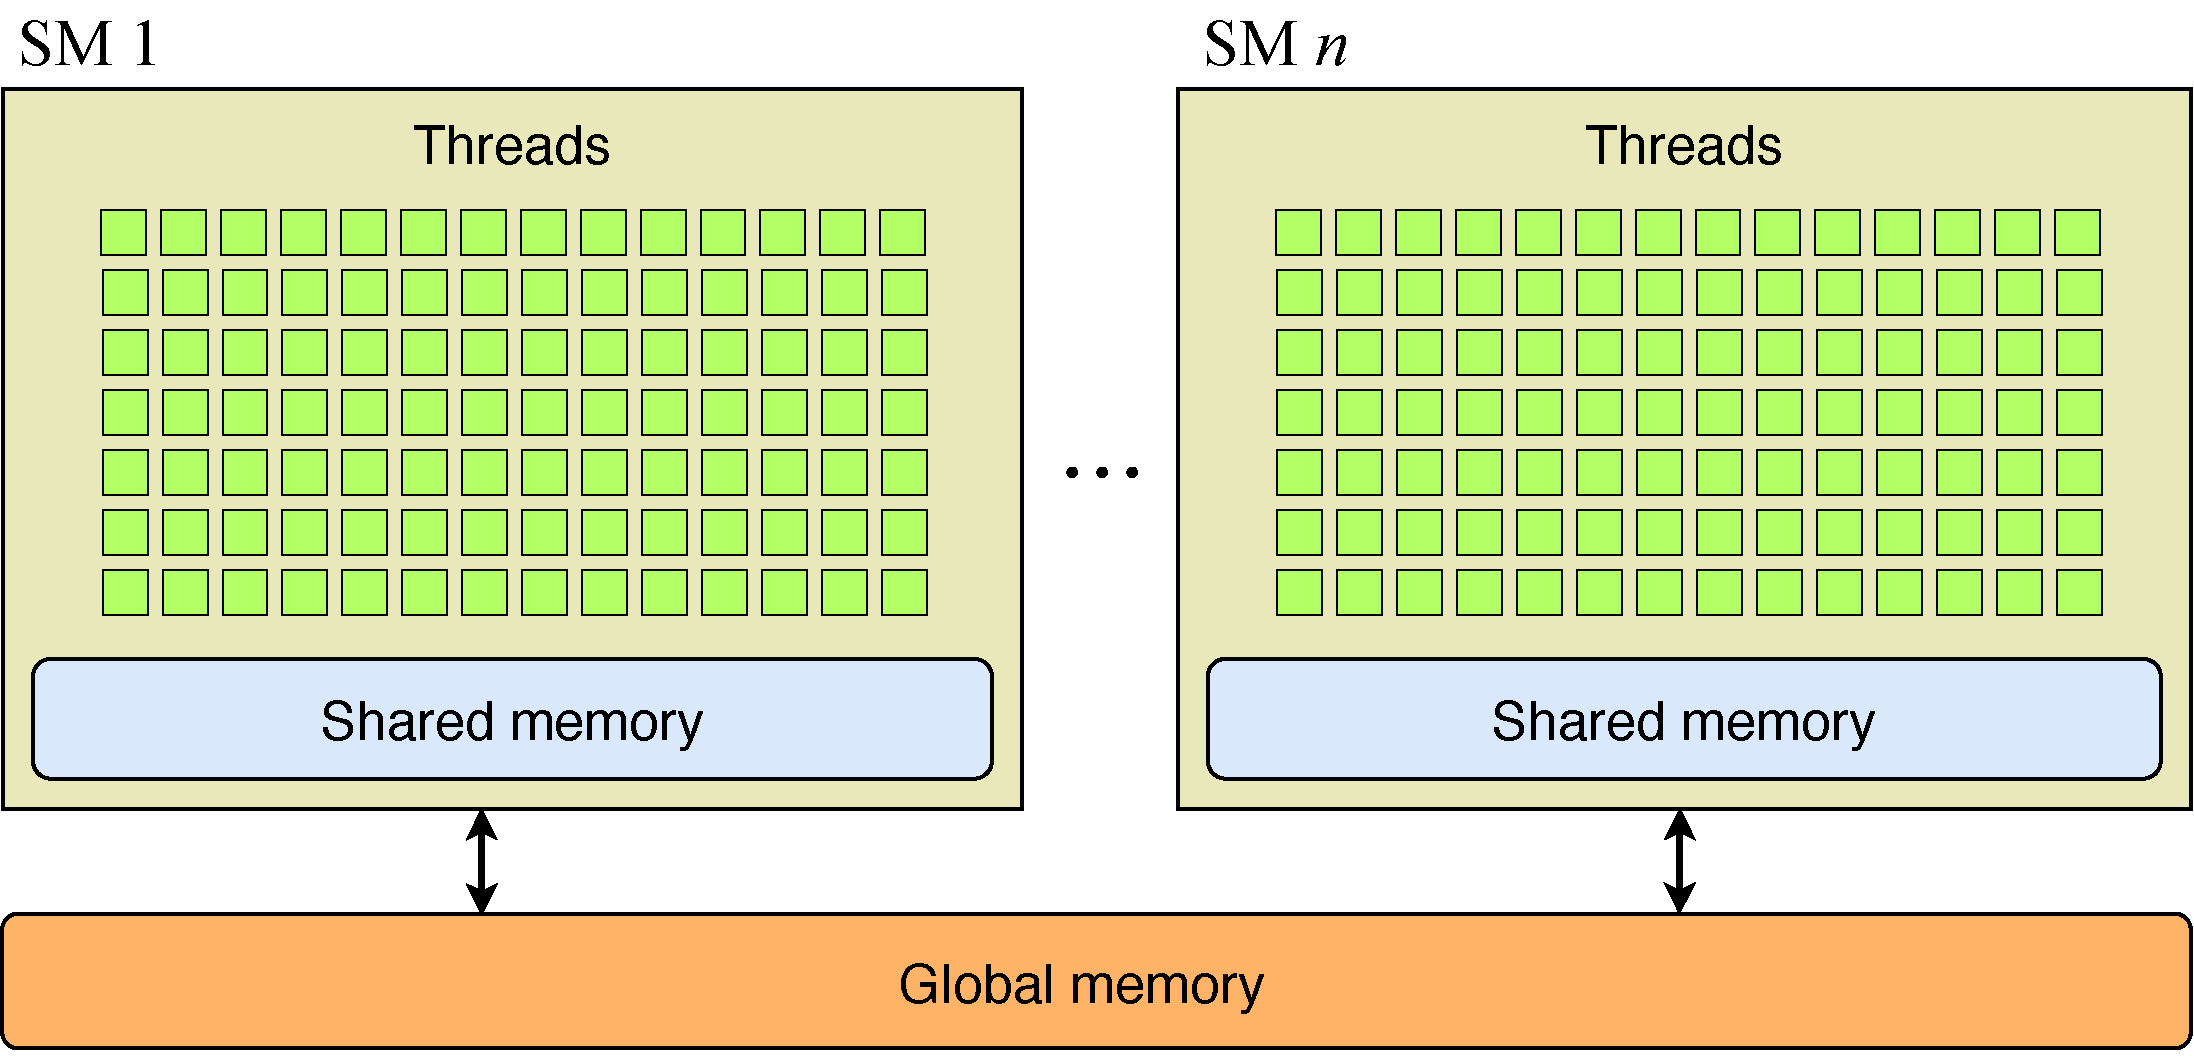
\includegraphics[width=\textwidth]{architecture.pdf}
	}
	\caption{GPU architecture.}
	\label{fig:gpu_architecture}
\end{figure}

We express a thread dimension with a bold italic font \td{dimension}. For example, threads or blocks can be launched in the \td{x} or \td{y} or \td{z} dimension. Additionally, in our developed kernels, we use two conventions. First of all, with \tx, we refer to the \emph{block-local} ID of the working thread in \td{x}. Second of all, we use so-called \emph{grid-stride loops} to process data elements in parallel. The statement \textbf{for all} $\tid \in \llbracket 0, N \rrbracket$ \textbf{do in parallel} expresses that all natural numbers in the range $[0,N)$ must be considered in the loop, and that this is done in parallel by having each executing thread start with element \tx, i.e., $\tid = \tx$, and before starting each additional iteration through the loop, the thread adds to \tid the total number of threads on the GPU. If the updated \tid is smaller than $N$, the next iteration is performed with this updated \tid. Otherwise, the thread exits the loop. A grid-stride loop ensures that when the range of numbers to consider is larger than the number of threads, all numbers are still processed.

\paragraph{Memory Hierarchy.}
A GPU has multiple types of memory. The largest of these is the \textit{global memory}. It can be used to copy data between the host and the device. It can be accessed by all GPU threads, and has a high bandwidth, but also a high latency. Other types are \emph{shared memory} and \emph{registers}. The former is on-chip memory with a low latency, that can be used as block-local memory; the threads of a block can share data with each other via this memory. Registers are the fastest, and is used to store thread-local data. Their size is very small, though, and allocating too much memory for thread-local variables may result in data spilling over into global memory, which can dramatically limit the performance.

GPU threads can also use atomic instructions to manipulate data atomically in both global and shared memory. For example \atomicXOR(\var{addr}, \var{val}) atomically \emph{xors} the memory location \var{addr} with 32-bit or 64-bit \var{val}. 

\section{Parallel Simulation on GPUs}

In this section we present the data structures and algorithms that we use for scheduling the simulation of parallel gates of Clifford circuits on GPUs by employing the stabilizers tableau formalism \cite{gottesman1997stabilizer}. In our parallel simulation algorithm, we perform two level of parallelism. On one level we sweep all parallel gates simultaneously at a specific time window. On the second level, we update all Pauli generators per gate in parallel. To handle two-level of parallelism, we use multi-dimensional kernel as discussed in Sect.\ref{sec:GPUProgramming}. More details on this in the subsequent sections \todo{reminder: point to the exact place}. 

The data structures and algorithms that we use are directly based on the stabilizer formalism \cite{gottesman1997stabilizer} but adapted for the highest possible performance on a GPU. After running comprehensive benchmarks for different architectural possibilities and evaluating their performance for the simulation of large Clifford circuits, we have established the architecture that we use at the optimal one given the limitations of current GPU technology. In the discussion that follows, we present a detailed description of our architecture and provide the necessary benchmarks to support our architectural choices.

\subsection{Parallel Gates Scheduling}

Let $n$ be the number of qubits. We call $\cliffordGroup_n = \{\text{H}_i,\text{S}_i,\text{CX}_{i,j} \mid i,j \in [n] \}$, the group of all Clifford gates acting on \numQubits qubits. Let the initial quantum state of a single qubit be $\ket{\qubit_1}$ such that $\qubit_1 \in \{0,1\}$. For two qubits, we have $\ket{\qubit_1\qubit_2} = \ket{\qubit_1}\otimes\ket{\qubit_2}$, where $\otimes$ is the tensor product. With $\wires(\newGate)$, we define the set of qubits (wires) attached to a Clifford gate $\newGate \in \mathcal{G}_n$ Based on the former notations, we define the set of parallel gates \circuitWindow as follows:

\begin{definition}[Parallel gates]\label{def:window}
	Given a set of Clifford gates $\mathcal{G}_n$, we call a set $\circuitWindow\subseteq\mathcal{G}_n$ a set of \emph{parallel gates} iff $\ \forall \newGate,\newGate'\in \circuitWindow.\ \wires(\newGate) \cap \wires(\newGate') = \emptyset$.
\end{definition}

\begin{figure}[t]
	\resizebox{1.1\textwidth}{!}{ 
	\begin{quantikz}
		\lstick{$\ket{q_0}$} & \gate{H}    & \gate{S}  &       & \qw          & \qw              & \ctrl{2}     & \qw   & \qw    & \qw           & \qw                   & \qw       &\qw            & \qw   & \qw  & \qw &\qw  &\qw \\
		\lstick{$\ket{q_1}$} & \qw    & \qw                            & \qw              & \qw                 &\gate{H}         & \qw    & \qw           & \qw     & \qw           & \qw            & \qw &\gate{H}   & \qw & \targ{3}    & \gate{S} & \qw   &\qw   \\
		\lstick{$\ket{q_2}$} & \qw    & \qw        & \gate{S}    & \qw     & \qw              &\targ{0}     & \qw      & \qw    & \qw                & \gate{H}               &\gate{H}    & \qw            & \qw     & \qw    & \qw  &\qw &\qw \\
		\lstick{$\ket{q_3}$} & \qw  & \qw         & \qw                     &  \gate{H} & \qw   & \qw                       &  \gate{S}        & \ctrl{1}    & \gate{S}                & \qw    & \qw & \qw  &\gate{S}                   & \ctrl{-2} &\qw  & \gate{S}  & \qw       \\
		\lstick{$\ket{q_4}$} & \qw & \qw  & \qw   & \qw           & \qw                                & \qw              & \qw              &  \targ{3}         & \qw                   & \qw                  & \qw    & \qw       & \qw    & \qw   & \qw  &\qw  &\qw \\
	\end{quantikz}
}\\\\


%% It's very conusing to introduce time windows concept on the initial circuit. Windows should appear on the resulting circuit.

%\begin{tikzpicture}[overlay]
%	\draw[ purple,line width=1.5pt, opacity=0.5] (0.95,4.2) -- (0.95,0.4); %the first vertical line
%	\draw[ purple,line width=1.5pt, opacity=0.5] (1.65,4.2) -- (1.65,0.4); %the second vertical
%	\draw[ purple,line width=1.5pt, opacity=0.5] (0.95,4.2) -- (1.65,4.2); %upper sealing
%	\draw[ purple,line width=1.5pt, opacity=0.5] (0.95,0.4) -- (1.65,0.4); %lower sealing
%	\node[anchor=north, text=purple, opacity=1] at (1.4,0.3) {$\circuitWindow_1$};
%	
%	
%	\draw[ purple,line width=1.5pt, opacity=0.5] (1.8,4.2) -- (1.8,0.4); %the first vertical line
%	\draw[ purple,line width=1.5pt, opacity=0.5] (2.5,4.2) -- (2.5,0.4); %the second vertical
%	\draw[ purple,line width=1.5pt, opacity=0.5] (1.8,4.2) -- (2.5,4.2); %upper sealing
%	\draw[ purple,line width=1.5pt, opacity=0.5] (1.8,0.4) -- (2.5,0.4); %lower sealing
%	\node[anchor=north, text=purple, opacity=1] at (2.2,0.3) {$\circuitWindow_2$};
%	
%	\node[anchor=north, text=purple, opacity=1] at (3,0.3) {$\cdots$};
%\end{tikzpicture}

{\centering
	\resizebox{0.575\textwidth}{!}{ 
		\begin{quantikz}
			\lstick{$\ket{q_0}$} & \gate{H}       & \gate{S}                        & \ctrl{2}     & \qw              & \qw               & \qw & \qw       &\qw       & \qw            \\
			\lstick{$\ket{q_1}$} & \gate{H}     
			& \gate{H}                          &  \qw        &\qw         & \qw             & \targ{3}      &\gate{S}  & \qw         & \qw      \\
			\lstick{$\ket{q_2}$} & \gate{S}      & \qw              &\targ{0}       & \gate{H}   & \gate{H}    &\qw   & \qw & \qw           & \qw  \\
			\lstick{$\ket{q_3}$} & \gate{H}           &  \gate{S}               & \ctrl{1}    & \gate{S}        & \gate{S}               &\ctrl{-2}      &\gate{S} & \qw    & \qw    \\
			\lstick{$\ket{q_4}$} & \qw   & \qw                                                      &  \targ{3}            & \qw   &\qw                 & \qw  & \qw          & \qw            & \qw  \\
		\end{quantikz}
	}\par
}

% Use if not centered
%\newcommand{\xCordLeft}{1}
%\newcommand{\xCordRight}{1.7}
\newcommand{\xCordLeft}{3.56}
\newcommand{\xCordRight}{4.25}
\newcommand{\yCordLow}{0.4}
\newcommand{\yCordHigh}{4.2}
\newcommand{\lineWidth}{1.5pt}
\newcommand{\lineOpac}{0.5}
\begin{tikzpicture}[overlay]
	\draw[ purple,line width=\lineWidth, opacity=\lineOpac] (\xCordLeft ,   \yCordHigh) -- (\xCordLeft,    \yCordLow); %the first vertical line
	\draw[ purple,line width=\lineWidth, opacity=\lineOpac] (\xCordRight,  \yCordHigh) -- (\xCordRight,  \yCordLow); %the second vertical
	\draw[ purple,line width=\lineWidth, opacity=\lineOpac] (\xCordLeft ,   \yCordHigh) -- (\xCordRight,  \yCordHigh); %upper sealing
	\draw[ purple,line width=\lineWidth, opacity=\lineOpac] (\xCordLeft ,   \yCordLow) -- (\xCordRight,   \yCordLow); %lower sealing
	\node[anchor=north, text=purple, opacity=1] at (3.9,0.3) {$\circuitWindow_1$};
	
%	\renewcommand{\xCordLeft}{1.85}
%	\renewcommand{\xCordRight}{2.55}
	\renewcommand{\xCordLeft}{4.4}
	\renewcommand{\xCordRight}{5.1}
	
	\draw[ purple,line width=\lineWidth, opacity=\lineOpac] (\xCordLeft ,   \yCordHigh) -- (\xCordLeft,    \yCordLow); %the first vertical line
	\draw[ purple,line width=\lineWidth, opacity=\lineOpac] (\xCordRight,  \yCordHigh) -- (\xCordRight,  \yCordLow); %the second vertical
	\draw[ purple,line width=\lineWidth, opacity=\lineOpac] (\xCordLeft ,   \yCordHigh) -- (\xCordRight,  \yCordHigh); %upper sealing
	\draw[ purple,line width=\lineWidth, opacity=\lineOpac] (\xCordLeft ,   \yCordLow) -- (\xCordRight,   \yCordLow); %lower sealing
	\node[anchor=north, text=purple, opacity=1] at (4.8,0.3) {$\circuitWindow_2$};

%	\renewcommand{\xCordLeft}{2.7}
%	\renewcommand{\xCordRight}{3.3}

	\renewcommand{\xCordLeft}{5.24}
	\renewcommand{\xCordRight}{5.9}
	
	\draw[ purple,line width=\lineWidth, opacity=\lineOpac] (\xCordLeft ,   \yCordHigh) -- (\xCordLeft,    \yCordLow); %the first vertical line
	\draw[ purple,line width=\lineWidth, opacity=\lineOpac] (\xCordRight,  \yCordHigh) -- (\xCordRight,  \yCordLow); %the second vertical
	\draw[ purple,line width=\lineWidth, opacity=\lineOpac] (\xCordLeft ,   \yCordHigh) -- (\xCordRight,  \yCordHigh); %upper sealing
	\draw[ purple,line width=\lineWidth, opacity=\lineOpac] (\xCordLeft ,   \yCordLow) -- (\xCordRight,   \yCordLow); %lower sealing
	\node[anchor=north, text=purple, opacity=1] at (5.6,0.3) {$\circuitWindow_3$};
	
	\node[anchor=north, text=purple, opacity=1] at (6.5,0.3) {$\cdots$};
\end{tikzpicture}

	\caption{Parsed circuit on the top. Scheduled circuit on the bottom.}
	\label{fig:circuit}
\end{figure}

The above definition is implemented on the host side such that we optain a maximal \circuitWindow of parallel gates. For this, we store the parsed Clifford circuit (top part of Fig.~\ref{fig:circuit}) in a FIFO queue. Then, we start with an empty \circuitWindow, and try to fill it with parallel gates that are removed from the queue until it's maximal length $|\circuitWindow| = \numQubits$ is reached or no more parallel gates can be assigned to \circuitWindow due to dependency. We repeat the former procedure, scheduling new \circuitWindow's untill the queue becomes empty (see the bottom part of Fig.~\ref{fig:circuit} for the end result). Thus, the queue can be only empty iff all gates are successfully scheduled to one or more \circuitWindow's which gurantees soundness (i.e. no gate is missed or misplaced) and termination.

%
%Alg.\ref{alg:scheduler} outlines an efficient way to schedule a set of parallel gates from a Clifford circuit with goal in mind not to cumbersome the parallel computations that run later on the GPU. It takes as input the number of qubits \numQubits and a FIFO queue \circuitQueue storing all gates parsed from a Clifford circuit in order of their appearence (See Fig.~\ref{fig:circuit}). That is, the first gate in \circuitQueue has the lowest depth level. The output is a set of windows where each window is a set of scheduled parallel gates. 
%
%\begin{figure}[t]
%	\resizebox{1.1\textwidth}{!}{ 
	\begin{quantikz}
		\lstick{$\ket{q_0}$} & \gate{H}    & \gate{S}  &       & \qw          & \qw              & \ctrl{2}     & \qw   & \qw    & \qw           & \qw                   & \qw       &\qw            & \qw   & \qw  & \qw &\qw  &\qw \\
		\lstick{$\ket{q_1}$} & \qw    & \qw                            & \qw              & \qw                 &\gate{H}         & \qw    & \qw           & \qw     & \qw           & \qw            & \qw &\gate{H}   & \qw & \targ{3}    & \gate{S} & \qw   &\qw   \\
		\lstick{$\ket{q_2}$} & \qw    & \qw        & \gate{S}    & \qw     & \qw              &\targ{0}     & \qw      & \qw    & \qw                & \gate{H}               &\gate{H}    & \qw            & \qw     & \qw    & \qw  &\qw &\qw \\
		\lstick{$\ket{q_3}$} & \qw  & \qw         & \qw                     &  \gate{H} & \qw   & \qw                       &  \gate{S}        & \ctrl{1}    & \gate{S}                & \qw    & \qw & \qw  &\gate{S}                   & \ctrl{-2} &\qw  & \gate{S}  & \qw       \\
		\lstick{$\ket{q_4}$} & \qw & \qw  & \qw   & \qw           & \qw                                & \qw              & \qw              &  \targ{3}         & \qw                   & \qw                  & \qw    & \qw       & \qw    & \qw   & \qw  &\qw  &\qw \\
	\end{quantikz}
}\\\\


%% It's very conusing to introduce time windows concept on the initial circuit. Windows should appear on the resulting circuit.

%\begin{tikzpicture}[overlay]
%	\draw[ purple,line width=1.5pt, opacity=0.5] (0.95,4.2) -- (0.95,0.4); %the first vertical line
%	\draw[ purple,line width=1.5pt, opacity=0.5] (1.65,4.2) -- (1.65,0.4); %the second vertical
%	\draw[ purple,line width=1.5pt, opacity=0.5] (0.95,4.2) -- (1.65,4.2); %upper sealing
%	\draw[ purple,line width=1.5pt, opacity=0.5] (0.95,0.4) -- (1.65,0.4); %lower sealing
%	\node[anchor=north, text=purple, opacity=1] at (1.4,0.3) {$\circuitWindow_1$};
%	
%	
%	\draw[ purple,line width=1.5pt, opacity=0.5] (1.8,4.2) -- (1.8,0.4); %the first vertical line
%	\draw[ purple,line width=1.5pt, opacity=0.5] (2.5,4.2) -- (2.5,0.4); %the second vertical
%	\draw[ purple,line width=1.5pt, opacity=0.5] (1.8,4.2) -- (2.5,4.2); %upper sealing
%	\draw[ purple,line width=1.5pt, opacity=0.5] (1.8,0.4) -- (2.5,0.4); %lower sealing
%	\node[anchor=north, text=purple, opacity=1] at (2.2,0.3) {$\circuitWindow_2$};
%	
%	\node[anchor=north, text=purple, opacity=1] at (3,0.3) {$\cdots$};
%\end{tikzpicture}

{\centering
	\resizebox{0.575\textwidth}{!}{ 
		\begin{quantikz}
			\lstick{$\ket{q_0}$} & \gate{H}       & \gate{S}                        & \ctrl{2}     & \qw              & \qw               & \qw & \qw       &\qw       & \qw            \\
			\lstick{$\ket{q_1}$} & \gate{H}     
			& \gate{H}                          &  \qw        &\qw         & \qw             & \targ{3}      &\gate{S}  & \qw         & \qw      \\
			\lstick{$\ket{q_2}$} & \gate{S}      & \qw              &\targ{0}       & \gate{H}   & \gate{H}    &\qw   & \qw & \qw           & \qw  \\
			\lstick{$\ket{q_3}$} & \gate{H}           &  \gate{S}               & \ctrl{1}    & \gate{S}        & \gate{S}               &\ctrl{-2}      &\gate{S} & \qw    & \qw    \\
			\lstick{$\ket{q_4}$} & \qw   & \qw                                                      &  \targ{3}            & \qw   &\qw                 & \qw  & \qw          & \qw            & \qw  \\
		\end{quantikz}
	}\par
}

% Use if not centered
%\newcommand{\xCordLeft}{1}
%\newcommand{\xCordRight}{1.7}
\newcommand{\xCordLeft}{3.56}
\newcommand{\xCordRight}{4.25}
\newcommand{\yCordLow}{0.4}
\newcommand{\yCordHigh}{4.2}
\newcommand{\lineWidth}{1.5pt}
\newcommand{\lineOpac}{0.5}
\begin{tikzpicture}[overlay]
	\draw[ purple,line width=\lineWidth, opacity=\lineOpac] (\xCordLeft ,   \yCordHigh) -- (\xCordLeft,    \yCordLow); %the first vertical line
	\draw[ purple,line width=\lineWidth, opacity=\lineOpac] (\xCordRight,  \yCordHigh) -- (\xCordRight,  \yCordLow); %the second vertical
	\draw[ purple,line width=\lineWidth, opacity=\lineOpac] (\xCordLeft ,   \yCordHigh) -- (\xCordRight,  \yCordHigh); %upper sealing
	\draw[ purple,line width=\lineWidth, opacity=\lineOpac] (\xCordLeft ,   \yCordLow) -- (\xCordRight,   \yCordLow); %lower sealing
	\node[anchor=north, text=purple, opacity=1] at (3.9,0.3) {$\circuitWindow_1$};
	
%	\renewcommand{\xCordLeft}{1.85}
%	\renewcommand{\xCordRight}{2.55}
	\renewcommand{\xCordLeft}{4.4}
	\renewcommand{\xCordRight}{5.1}
	
	\draw[ purple,line width=\lineWidth, opacity=\lineOpac] (\xCordLeft ,   \yCordHigh) -- (\xCordLeft,    \yCordLow); %the first vertical line
	\draw[ purple,line width=\lineWidth, opacity=\lineOpac] (\xCordRight,  \yCordHigh) -- (\xCordRight,  \yCordLow); %the second vertical
	\draw[ purple,line width=\lineWidth, opacity=\lineOpac] (\xCordLeft ,   \yCordHigh) -- (\xCordRight,  \yCordHigh); %upper sealing
	\draw[ purple,line width=\lineWidth, opacity=\lineOpac] (\xCordLeft ,   \yCordLow) -- (\xCordRight,   \yCordLow); %lower sealing
	\node[anchor=north, text=purple, opacity=1] at (4.8,0.3) {$\circuitWindow_2$};

%	\renewcommand{\xCordLeft}{2.7}
%	\renewcommand{\xCordRight}{3.3}

	\renewcommand{\xCordLeft}{5.24}
	\renewcommand{\xCordRight}{5.9}
	
	\draw[ purple,line width=\lineWidth, opacity=\lineOpac] (\xCordLeft ,   \yCordHigh) -- (\xCordLeft,    \yCordLow); %the first vertical line
	\draw[ purple,line width=\lineWidth, opacity=\lineOpac] (\xCordRight,  \yCordHigh) -- (\xCordRight,  \yCordLow); %the second vertical
	\draw[ purple,line width=\lineWidth, opacity=\lineOpac] (\xCordLeft ,   \yCordHigh) -- (\xCordRight,  \yCordHigh); %upper sealing
	\draw[ purple,line width=\lineWidth, opacity=\lineOpac] (\xCordLeft ,   \yCordLow) -- (\xCordRight,   \yCordLow); %lower sealing
	\node[anchor=north, text=purple, opacity=1] at (5.6,0.3) {$\circuitWindow_3$};
	
	\node[anchor=north, text=purple, opacity=1] at (6.5,0.3) {$\cdots$};
\end{tikzpicture}

%	\caption{Parsed circuit on the top. Scheduled circuit on the bottom.}
%	\label{fig:circuit}
%\end{figure}
%
%\begin{algorithm}[t]
%	\DontPrintSemicolon
%	\caption{Parallel gates scheduler.}
%	\label{alg:scheduler}
%	\footnotesize
%	\SetCommentSty{mycommfont}
%	\SetArgSty{}
%	\SetKwInput{Input}{Input~}
%	\SetKwInput{Output}{Output~}
%	\KwIn{\circuitQueue, \numQubits}
%	\KwOut{\circuitScheduled}
%		$\circuitScheduled \gets \emptyset$ \label{l:initScheduled} \tcp*[r]{Set of scheduled windows.}
%		\While{$\circuitQueue \neq \emptyset$}{ \label{l:depthLoop} 
%			$\circuitWindow \gets \emptyset$ \label{l:initWindow} \tcp*[r]{Set of parallel gates per window.}
%			$\lockedSet \gets \emptyset$,\ $\numQubits' \gets 0$  \label{l:initLocked} \tcp*[r]{Set of locked qubits and its old size.}
%			\While{$\circuitQueue \neq \emptyset$}{ \label{l:windowLoop} 
%				$\newGate \gets \pickFront$($\circuitQueue$)\; \label{l:pickFront}
%				\If(\tcp*[f]{Are all qubits in \newGate unlocked?}){$\wires(\newGate) \not\subseteq \lockedSet$}{ \label{l:checkunlocked} 
%					$\circuitWindow \gets \circuitWindow \cup \newGate$,\ \label{l:addGate} 
%					$\circuitQueue \gets \circuitQueue \setminus \newGate$ \label{l:removeGate} \tcp*[r]{Found new parallel gate.}
%					$\lockedSet \gets \lockedSet \cup \wires(\newGate)$ \label{l:lockQubitNewGate} \tcp*[r]{lock new qubits.}
%				}
%				\Else{ \label{l:checkunlockedElse} 
%					$\lockedSet \gets \lockedSet \cup \wires(\newGate)$ \label{l:lockQubit} \tcp*[r]{lock new qubits.}
%				}
%				\If(\tcp*[f]{Fixpoint for forced termination.}){$|\lockedSet| = \numQubits \vee |\lockedSet| = \numQubits'$} { \label{l:fixpoint}
%					$\Break$ \label{l:break}
%				} 
%				$\numQubits' = |\lockedSet|$ \label{l:recordLocked} \tcp*[r]{Record the last number of locked qubits.}
%			}
%			$\circuitScheduled \gets \circuitScheduled \cup \circuitWindow$	\label{l:addWindow} \tcp*[r]{Schedule new window.}
%		}
%
%\end{algorithm}
%
%Initially, at l.\ref{l:initScheduled}, \circuitScheduled is set to $\emptyset$. The outer loop at l.\ref{l:depthLoop} tries to assign a new window to \circuitScheduled as long as there are gates pending in \circuitQueue.  At l.\ref{l:initWindow}-\ref{l:initLocked}, we initialize a new window \circuitWindow and a set of locked gates \lockedSet. The notation $\numQubits'$ denotes the old size of \lockedSet. The inner loop at l.\ref{l:windowLoop} scans all gates in \circuitQueue and tries to assign a new parallel gate into \circuitWindow. The reason for the inner loop is to restrict the size of the current window $|\circuitWindow|$ to at most \numQubits. If the circuit queue had gates more than \numQubits (i.e. multiple depth levels) while the outer loop gurantees that all gates are scheduled to different windows. At l.\ref{l:pickFront}, the first gate in \circuitWindow is picked. If  l.\ref{l:checkunlocked} evaluates true (see Def.\ref{def:window}) then \newGate is a parallel gate and can be scheduled into \circuitWindow. After \newGate is added to \circuitWindow, we remove it from the queue \circuitWindow and lock all its qubits (l.\ref{l:lockQubitNewGate}) to prevent scheduling it again in the next window. If there is (at least one) qubit locked, all other qubits are locked at l.\ref{l:lockQubit}. To better explain when l.\ref{l:checkunlockedElse} is reached, consider the following scenario: 1-qubit gate such as H($5$) is scheduled at some iteration and its qubit $5$ is locked. Next, the gate CX($5, 6$) is fetched from the queue. Clearly, CX is not scheduled due to the shared qubit $5$, hence lines \ref{l:addGate}-\ref{l:lockQubitNewGate} are not executed. If the other qubit $6$ is missed from locking, the total number of locked qubits deemed inaccurate and the two conditions at l.\ref{l:fixpoint} will never hold. These conditions act as a termination fixpoint to exit the inner loop in case the queue still has gates to schedule. The fixpoint holds iff all qubits are locked or the previous number of locked qubits did not change (recorded at l.\ref{l:recordLocked}). The latter condition prevents stagnation if there are empty wires in the circuits without attached gates.  
%Next we prove through the following Lemmas and Theorems that Alg.\ref{alg:scheduler} is sound and terminates.
%
%\begin{lemma}\label{lem:correct1}
%	The order of gates per wire in the scheduled circuit \circuitScheduled is preserved and strictly follows the order of the original circuit.
%\end{lemma}
%
%\begin{proof}
%	Since the original circuit is stored in a FIFO queue and ordered w.r.t their appearance in the circuit depth (see Fig.\ref{fig:circuit}), l.\ref{l:pickFront} will always pick the first gate appeared on a wire with the lowest depth level. Thus, all parallel gates added to a new window at l.\ref{l:addGate} strictly follows the same order of the queue hence the original circuit. \qed
%\end{proof}
%
%\begin{lemma}\label{lem:terminate1}
%	Every time the inner loop at l.\ref{l:windowLoop} is entered, l.\ref{l:addWindow} is eventually reached with $1 \leq |\circuitWindow| \leq \numQubits$.
%\end{lemma}
%
%\begin{proof}
%	It follows from the outer loop at l.\ref{l:depthLoop} that the inner loop at l.\ref{l:windowLoop} is only entered iff the circuit queue \circuitQueue has at least one gate ($\circuitQueue \neq \emptyset$). Hence l.\ref{l:pickFront} is executed and a new gate \newGate is fetched. At this point two scenarios are possible: 1) \newGate has no locked qubits and l.\ref{l:addGate}-\ref{l:lockQubitNewGate} are reached; Hence, \newGate is added to \circuitWindow (e.g. \newGate is a parallel gate) and its qubits are locked.  2) At least one qubit is locked which implies that one or more gates were previously added to \circuitWindow. That is, $|\circuitWindow| \geq 1$. If the number of locked qubits $|\lockedSet|$ reaches \numQubits, l.\ref{l:fixpoint} will hold via the condition $|\lockedSet| = \numQubits$ and the break statement at l.\ref{l:break} is hit. Otherwise, the current number of locked qubits is recorded at l.\ref{l:recordLocked}. If that number does not change, the check $|\lockedSet| = \numQubits'$ holds and l.\ref{l:break} is hit. Thus, l.\ref{l:addWindow} is eventually reached with $1 \leq |\circuitWindow| \leq \numQubits$. \qed
%\end{proof}
%
%\begin{lemma}\label{lem:terminate2}
%	Alg.\ref{alg:scheduler} eventually terminates and $0 \leq |\circuitScheduled| \leq |\circuitQueue|$ always holds.
%\end{lemma}
%
%\begin{proof}
%	Initially, we have $\circuitScheduled = \emptyset$. If \circuitQueue is empty, the loop at l.\ref{l:depthLoop} is not entered and we have $|\circuitScheduled|  = 0$. If \circuitQueue has at least one gate then it follows from Lemma\ref{lem:terminate1} that l.\ref{l:addWindow} is eventually reached with $1 \leq |\circuitWindow| \leq \numQubits$. Since the outer loop at l.\ref{l:depthLoop} will never exit as long as the queue \circuitQueue is not empty, Alg.\ref{alg:scheduler} only terminates iff all gates in \circuitQueue are  scheduled and added to at least one window. In worst case scenario, all gates are sharing the same qubit and hence $|\circuitScheduled| = |\circuitQueue|$. Otherwise, we have $|\circuitScheduled| < |\circuitQueue|$ if $|\circuitWindow| > 1$. Therefore, in general, $0 \leq |\circuitScheduled| \leq |\circuitQueue|$ always holds. \qed
%\end{proof}
%
%\begin{theorem}\label{th:scheduler}
%	Alg.\ref{alg:scheduler} is sound and terminates.
%\end{theorem}
%
%\begin{proof}
%	It immediately follows from Lemmas \ref{lem:correct1}, \ref{lem:terminate1} and \ref{lem:terminate2} that both loops at l.\ref{l:depthLoop} and l.\ref{l:windowLoop}  can only terminate iff $\circuitQueue = \emptyset$ with $0 \leq |\circuitScheduled| \leq |\circuitQueue|$. Thus, $\{\newGate \mid \forall \circuitWindow \in \circuitScheduled. \newGate \in \circuitWindow\} = \{\newGate \mid \newGate \in \circuitQueue\}$ always holds. That is, Alg.\ref{alg:scheduler} schedules all gates from the original circuit (while preserving gate precedency) to one or more windows without missing any gate and only then it can terminate. \qed
%\end{proof}

\subsection{Data structure and Memory layout}

In this section, we discuss our architectural choices to optimally store/access parallel gates and tableau generators in GPU memory. Fig.\ref{fig:ds} shows our proposed data structures denoted as \code{Gate}, \code{Window}, and \code{Tableau}. The \code{Gate} structure requires at least 4 bytes of bookkeeping for the gate \code{type} (e.g. H, S, etc.) and \code{size} (number of qubits per gate). Even though both members are defined as bytes, the C standard defines a minimum of 4-byte memory alignment for \code{struct} data types. In addition, we have a flexible array \code{qubits[0]} to dynamically store gate wires or qubits. In total, a gate occupies $4 + 4\times \code{size}$ bytes. The \code{gates} field in \code{Window} (Fig. \ref{fig:window}) stores the raw bytes of \code{Gate} instances with any extra qubits in 4-byte buckets with 32-bit reference. The \code{cap} variable indicates the total memory capacity available for the storage of gates, and \code{size} reflects the current window size, i.e., number of parallel gates. We always have $\code{size} \leq \code{cap}$. The \code{references} field is used to directly access the gates by saving for each gate a reference to their first bucket. 

The \code{Tableau} structure contains fields resembling the \code{x}, \code{z}, and \code{signs} matrices. Each matrix is stored as column-major in memory (same layout as the original tableau \todo{reference to the prelims}) where \code{width} denote the number of qubits \numQubits and \code{height} denotes the number of generators' words of type \code{word\_t}. Typically, the matrix size of \code{x} and \code{z} is $\numQubits \times (\numQubits / \routine{sizeof}(\code{word\_t}))$ words. While the size of \code{signs} is $\numQubits / \routine{sizeof}(\code{word\_t})$ words.
To reduce memory footprint and run time, A \code{word\_t} word should span a group of generator bits to allow the execution of single operation on multiple generators at once. Based on the benchmarks in Fig.\ref{fig:words} over random circuits with thousands of qubits, we found out that 64-bit word is optimal. Further, as shown by Fig.\ref{fig:interleaving}, storing \code{x} and \code{z} matrices separately is arguably better than interleaving them in one matrix. This might seem surprising at first, since for the simulation of Hadamard gates, for which communication between the \code{x} and \code{z} matrices is required, it would mean maximal data latency. But for gates other than Hadamard, there is no communication between the \code{x} and \code{z} matrices, meaning that interleaving increases the data latency for those operations making the two architectural choices practically equivalent.

\newcommand{\gateW}{0.35}
\newcommand{\windowW}{0.35}
\newcommand{\tableauW}{0.35}
\begin{figure*}[t!]
	\centering
	\adjustbox{max width=\linewidth} {
		\subfloat[container for a gate]{
			\label{fig:gate}
			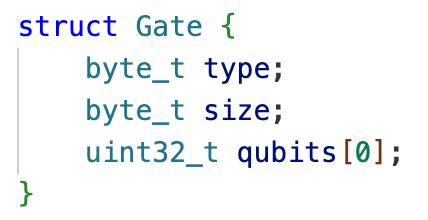
\includegraphics[width=\gateW\linewidth]{gate_container.png}
		} 
		\quad
		\subfloat[container for a window]{
			\label{fig:window}
			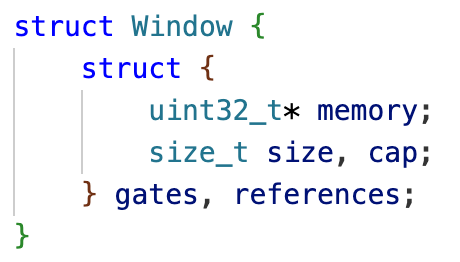
\includegraphics[width=\windowW\linewidth]{window_container.png}
		} 
		\quad
		\subfloat[container for a tableau]{
			\label{fig:tableau}
			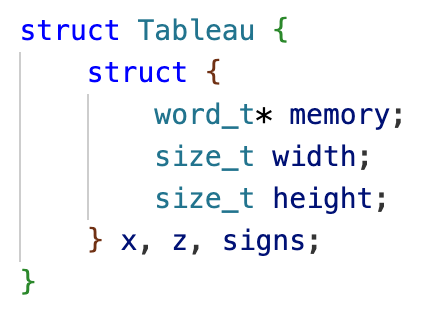
\includegraphics[width=\tableauW\linewidth]{tableau_container.png}
		} 
	}
	\caption{Data structures to store parallel gates and tableau generators.}
	\label{fig:ds}
\end{figure*}

\begin{figure*}[!t]
	\centering
	\adjustbox{max width=\linewidth} {
		\captionsetup[subfloat]{labelfont=large,textfont=large}
		\subfloat[different word sizes of 8, 32, and 64 bits]{
			\label{fig:words}
			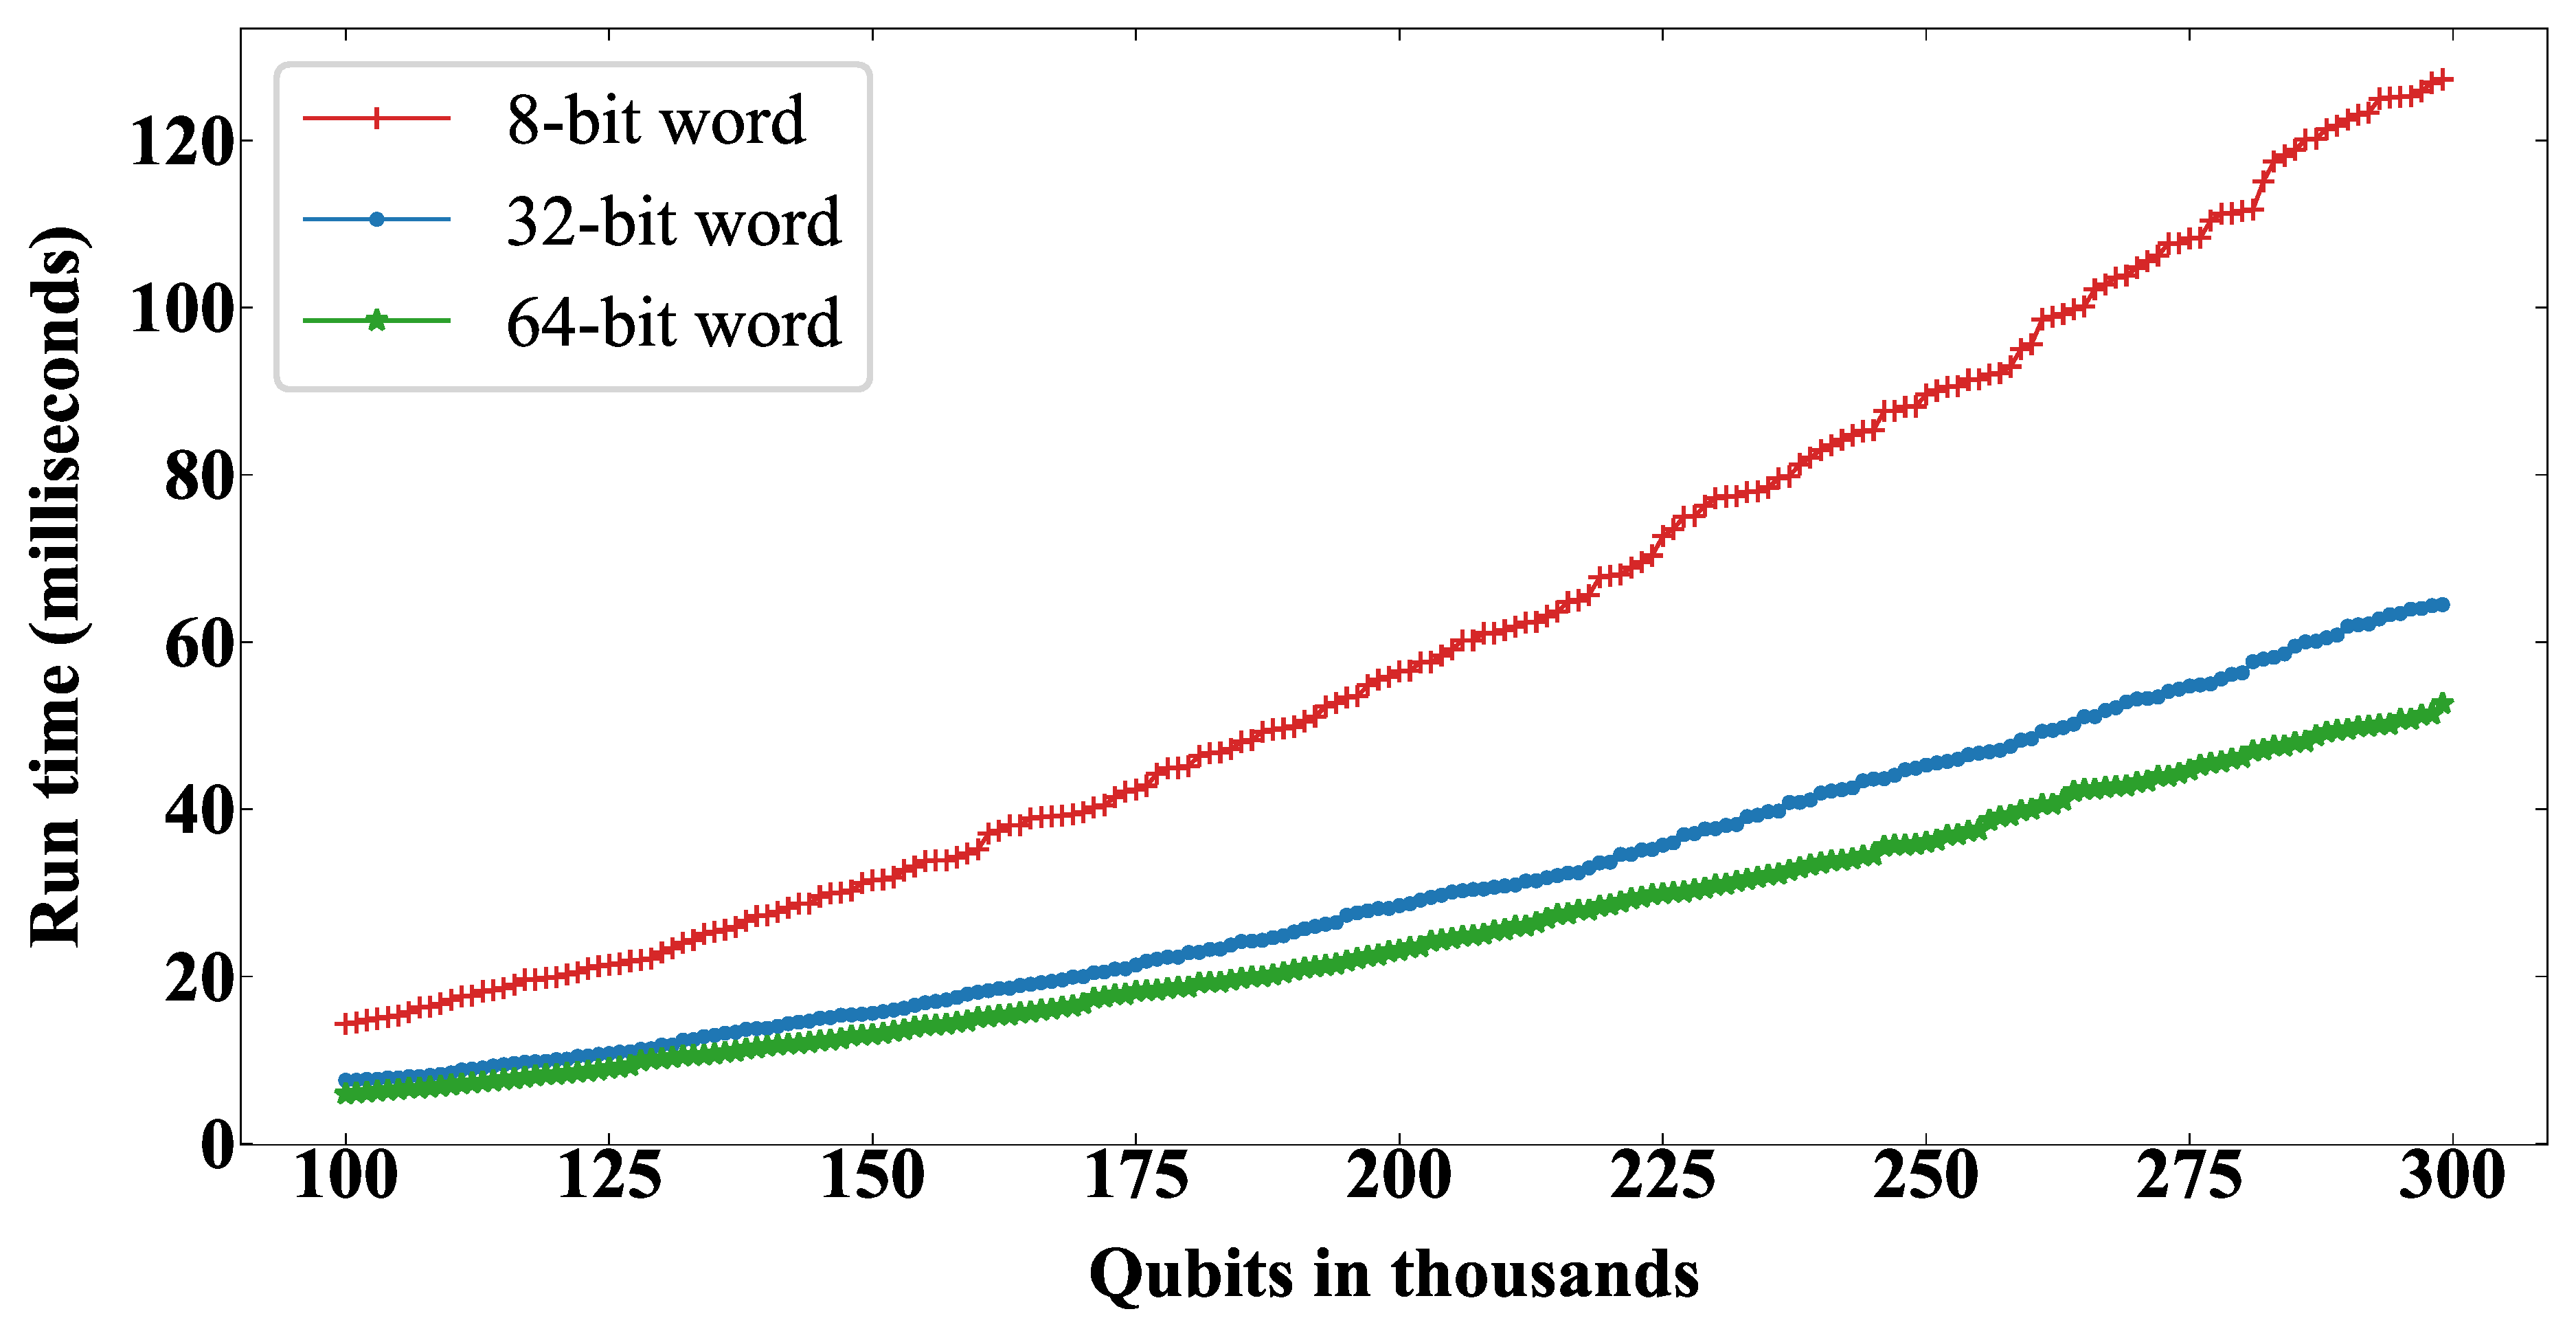
\includegraphics[width=\linewidth]{time_words.pdf}
		}
		\quad
		\subfloat[tableau interleaving vs no-interleaving]{
			\label{fig:interleaving}
			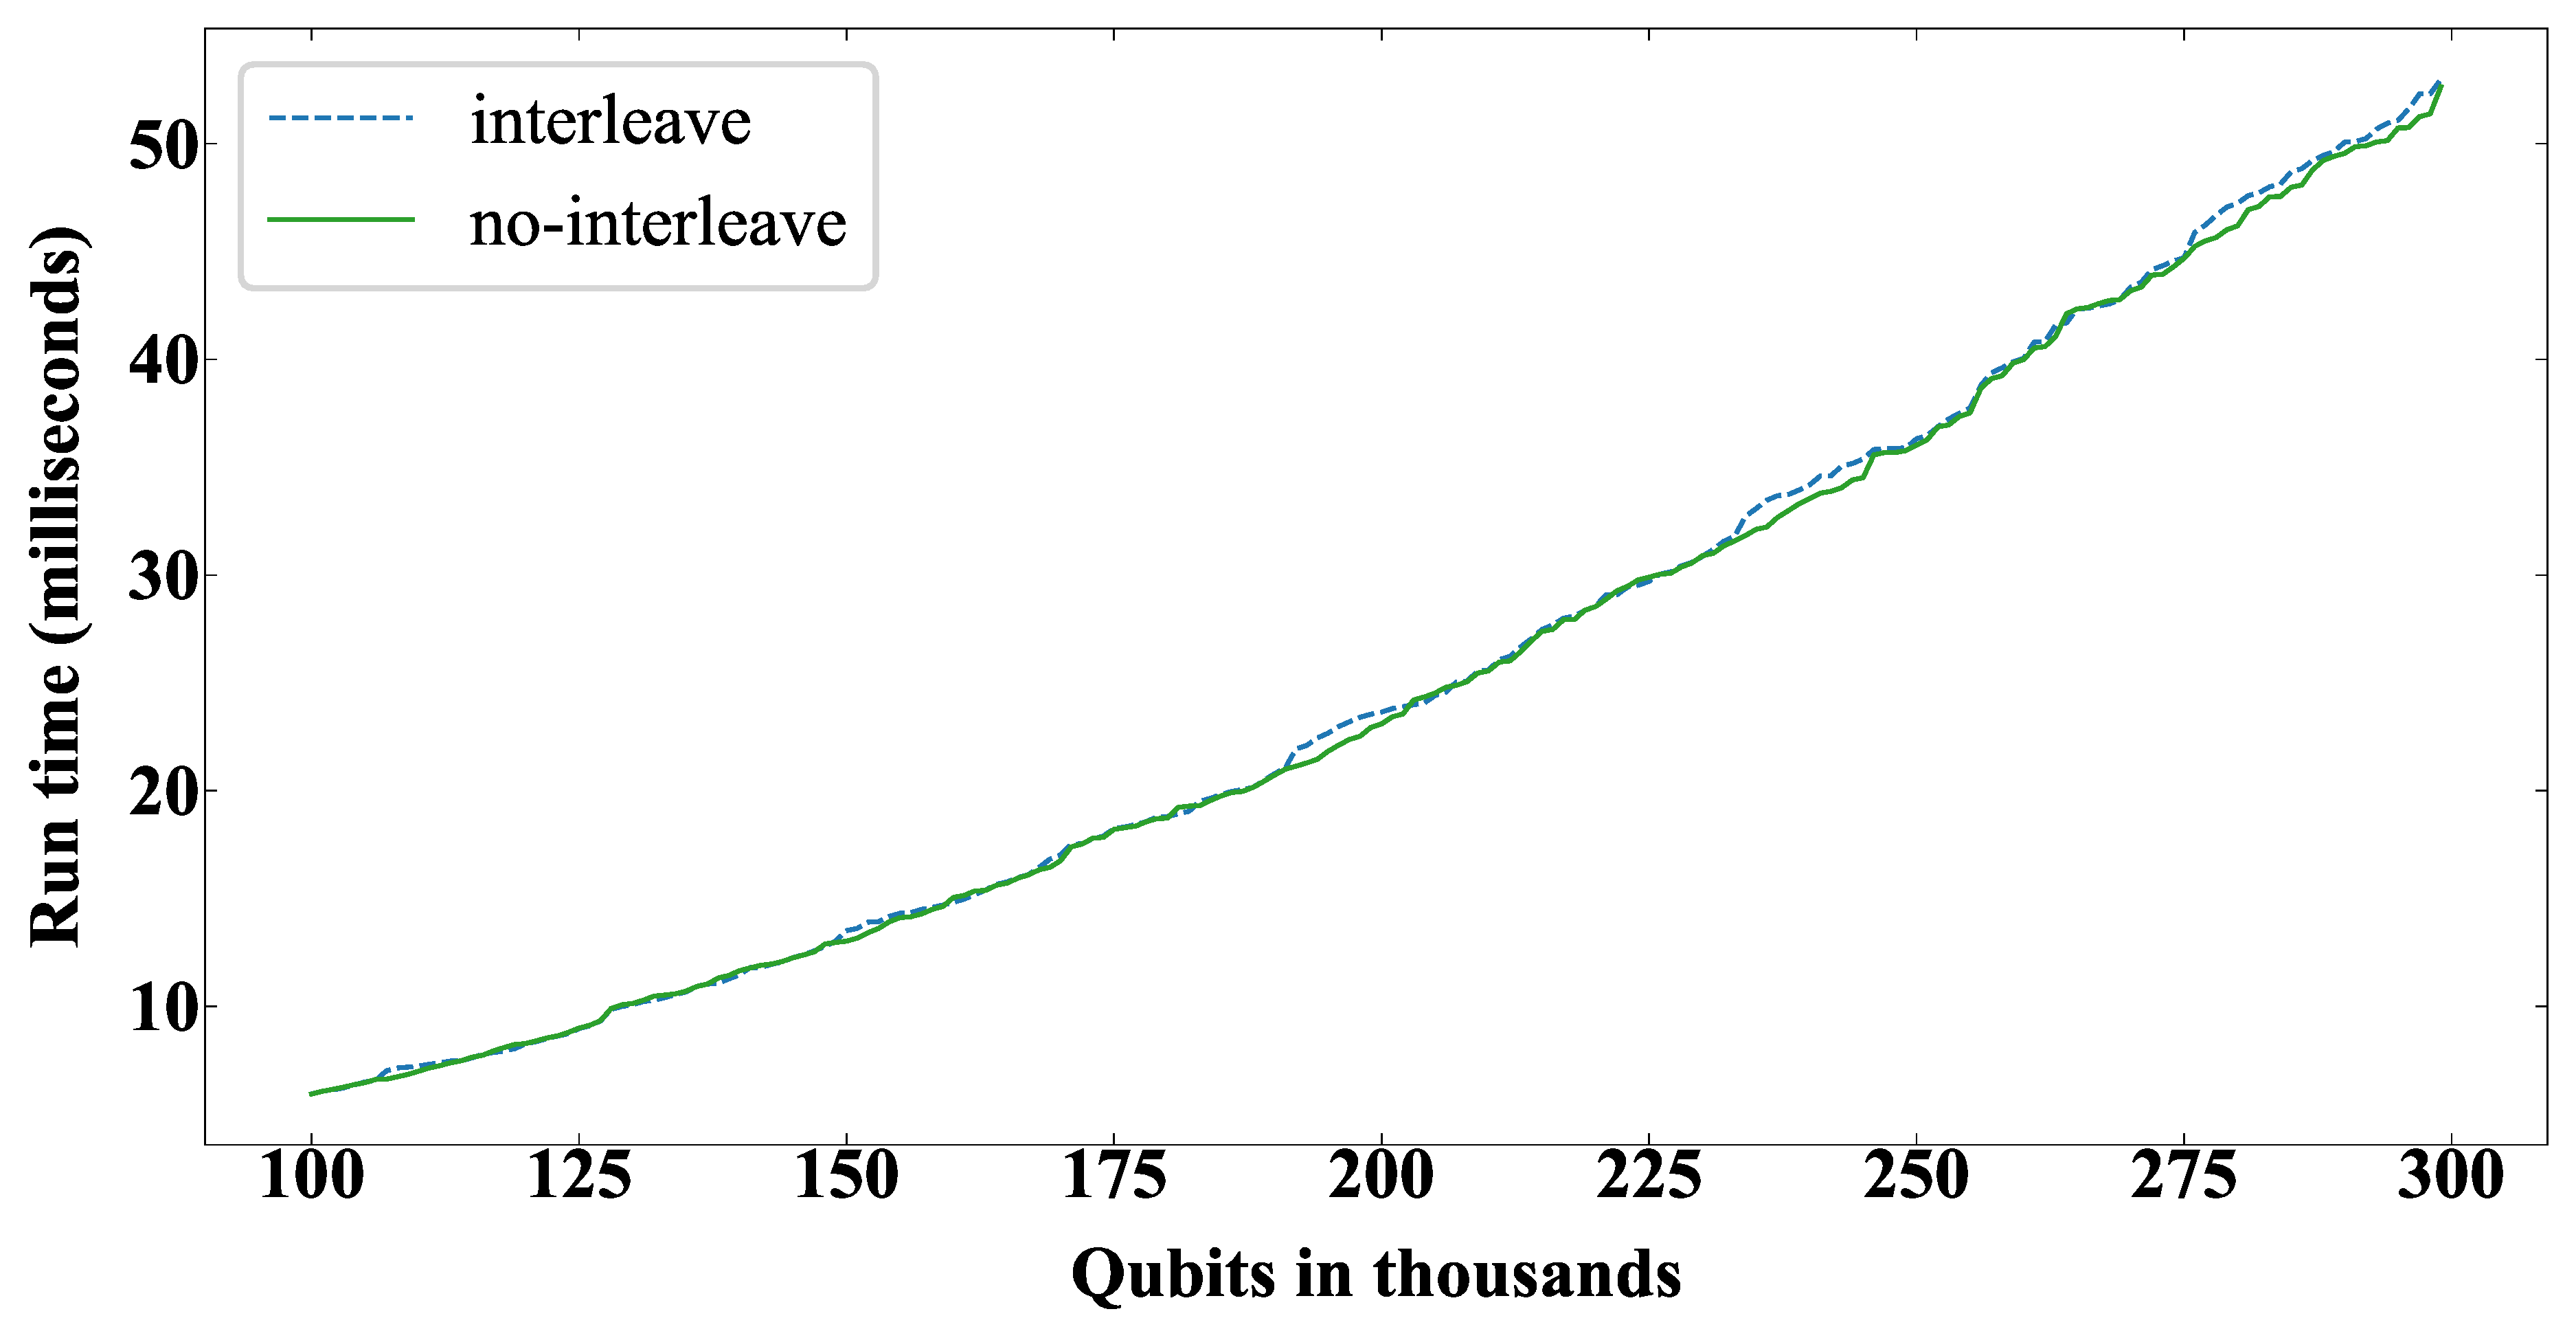
\includegraphics[width=\linewidth]{time_interleave.pdf}
		} 
	}
	\caption{Performance impact of different architectural choices.}
	\label{fig:configs}
\end{figure*}

\subsection{Stabilizers Tableau Partitioning}
 
Memory on GPUs is a scarce resource especially if the problem size is exponentially growing. For an XZ tableau encoding \numQubits qubits in Clifford circuits, we need $2\numQubits^{2} + \numQubits/ 8 $ bytes. For example, 1 million qubits would require 250 GB of GPU memory to store the tableau. This is even a challenge for CPU system memory. To tackle this, we propose a technique to safely slice the tableau into non-square partitions while keeping the computations integrity intact. Out technique allows simulating quantum circuits with millions of qubits using only the available memory no matter the size. 

The new partition size is $\tableauHeight \times \tableauWidth$ where \tableauHeight is the number of rows, i.e., the tableau is updated for all qubits but only for \tableauHeight generators. The \tableauHeight parameter is tuned down for a value $\tableauHeight < \numQubits$ such that the available memory is completely occupied. Once the number of partitions is determined, next step is to initialize the partitions to the same initial state of the original tableau. Fig. \ref{fig:partitions} shows an example of a tableau broken into two partitions and initialized to identity matrix to encode the state $\ket{0000}$. Note the offset of ones in the second partition by $\tableauHeight = 2$ columns, that is, for the $\partition\text{-th}$'s partition, the offset is $(\partition -  1)\tableauHeight$.

\todo{in figure \ref{fig:partitions} must change 0s and 1s to words, i.e. $w_{i,j}$} 
\begin{figure}[t]
	\centering
	\adjustbox{max width=\textwidth}{
		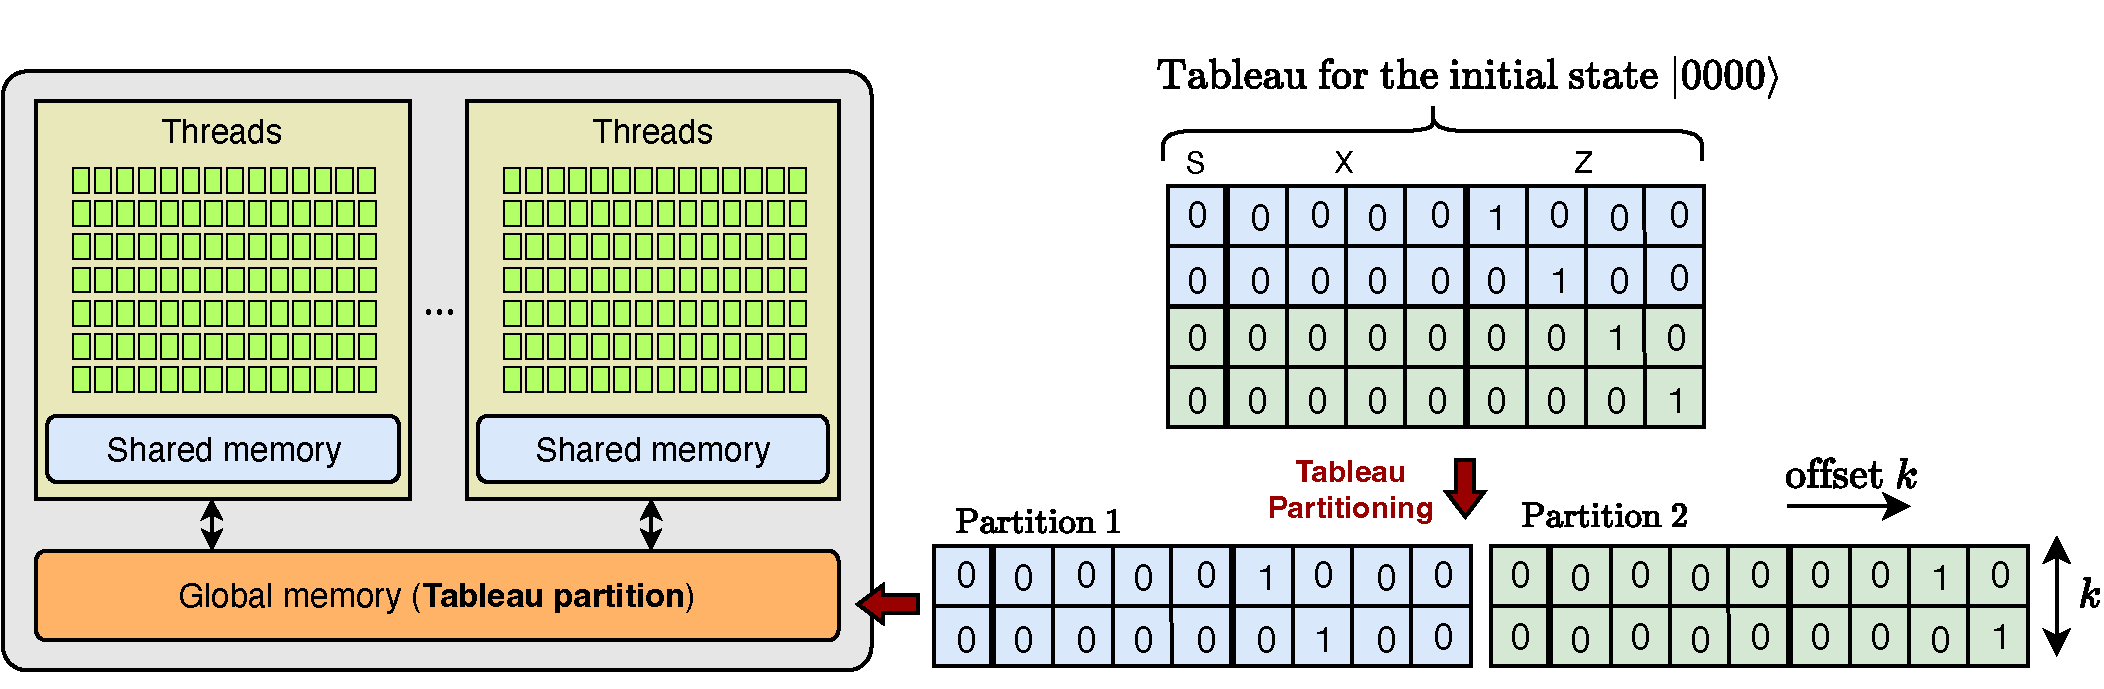
\includegraphics[width=\textwidth]{Partitions.pdf}
	}
	\caption{Tableau partitioning example of 4-qubit state.}
	\label{fig:partitions}
\end{figure}

\todo{Tableau/Partition should span at least 1 word (8-packed bits). Bit packing will be briefly explained earlier.}

\subsection{Tree-based Parallel Simulation on GPUs}

\todo[inline]{The notation here is not consistent with the prior text}

After we obtain the scheduled circuit \circuitScheduled from Alg.\ref{alg:scheduler}, we run Alg.\ref{alg:simulator} to iterate over each window $\circuitWindow \in \circuitScheduled$ and dispatch a GPU kernel that scans all parallel gates in $\circuitWindow$ and update the stabilizer tableau $\tableauPartition$ accordingly. 
First of all, at \li{ll:copyCircuit}, the whole scheduled circuit is copied asynchronously to the device. Asynchronous data transfer allows the host to immediately move to the next instruction without waiting for the transfer to complete. For example, the tableau allocation and partitioning can proceed at \li{ll:allocTableau} while the circuit transfer is pending. If the tableau fits entirely into the GPU memory, then the values of \numPartitions and \tableauHeight will be 1 resp. \numQubits. Otherwise, $\numPartitions$ is some value $>1$ such that $0 < \tableauHeight < \numQubits$. For simplicity, from now on, we refer by tableau $\tableauPartition$ to either a partition or the entire tableau.
Once the allocation is done and the values of \numPartitions and \tableauHeight are determined, we can synchronize the data transfer in \li{ll:syncHost}. 
The loop at \li{ll:forPartitions} simulate circuit $\circuitScheduled_d$ per partition $\partition$. This is done by first initializing $\tableauPartition$ to the quantum initial state at \li{ll:initTableau} offset by $(\partition - 1) \times \tableauHeight$, then the kernel \simulateWindow is launched to update the tableau for every $\circuitWindow_d \in \circuitScheduled_d$.

\begin{algorithm}[t]
	\setstretch{1.15}
	\DontPrintSemicolon
	\caption{Tree-based Parallel Simulation.}
	\label{alg:simulator}
	\scriptsize
	\SetCommentSty{mycommfont}
	\SetArgSty{}
	\SetKwInput{Input}{Input~}
	\SetKwInput{Output}{Output~}
	\KwIn{\circuitScheduled, \numQubits}
	\KwOut{\tableauPartition}
	$\circuitScheduled_d \gets \copyToDevice$($\circuitScheduled$) \label{ll:copyCircuit} \tcp*[r]{$\circuitScheduled_d$ resides in GPU memory.}
	$\tableauPartition,\ \tableauHeight,\ \numPartitions$ $\gets \allocate$($\numQubits$) \label{ll:allocTableau}	\tcp*[r]{$\tableauPartition$ is a tableau partition.}
	$\sync$() \label{ll:syncHost} \tcp*[r]{Synchronize with host side.}
	\ForEach{$\partition: 1 \to \numPartitions$}{ \label{ll:forPartitions} 
		\begingroup \color{gpu}
		$\tableauPartition \gets \initTableau$($\tableauPartition, (\partition - 1) \times \tableauHeight$) \label{ll:initTableau}  \tcp*[r]{Default: $\ket{0}^{\numQubits}$}
		\endgroup
		\ForAll{$\circuitWindow_d \in \circuitScheduled_d$}{ \label{ll:forWindow} 
			\begingroup \color{gpu}
			$\tableauPartition \gets \simulateWindow$($\tableauPartition, \circuitWindow_d, \tableauHeight$) \label{ll:simWindow}  \tcp*[r]{Simulate on GPU to obtain $\tableauPartition(\circuitWindow_d)$.}
			\endgroup
		}
	}
	\tcc{A 2D kernel to update the stabilizer tableau for a time window ($\circuitWindow_d$).}
	\begingroup \color{gpu}
	\Kernel{\upshape{\simulateWindow}($\tableauPartition, \circuitWindow_d, \tableauHeight$)}{  \label{ll:simWindowKernel} 
		$X \gets \tableauPartition^x,\ Z \gets \tableauPartition^z,\ S \gets \tableauPartition^s$ \label{ll:getMatrices}  \tcp*[r]{$X, Z, \text{and}\ S\ \text{are matrices in }\tableauPartition$.}
		\Forpary{$0, \tableauHeight$}{ \label{ll:forGenerators} 
			$\sign \gets S[\tidy],\ x \gets X[\tidy], z \gets Z[\tidy]$ \tcp*[r]{Thread $\tidy$ fetches a new row.}  \label{ll:getRow} 
			\Forparx{$0, |\circuitWindow_d|$}{ \label{ll:forGates} 
				$\parGate \gets \circuitWindow_d[\tidx]$ \tcp*[r]{Thread $\tidx$ fetches a new gate.}  \label{ll:getGate} 
				\Switch{$\parGate$}{ \label{ll:switch} 
					\lCase{H}{ \label{ll:H} 
						$\qubit \gets \wires(\text{H})$, 
						$\sign= \sign \oplus (x_{q} \wedge z_{q})$, 
						{\Swap}($x_{q}, z_{q}$)
					}
					\lCase{S}{ \label{ll:S} 
						$\qubit \gets \wires(\text{S})$, 
						$\sign= \sign \oplus (x_{q} \wedge z_{q})$, 
						$z_{q} \gets  z_{q} \oplus x_{q}$
					}
					\lCase{CX}{ \label{ll:CX} 
						$\qubit_1,\ \qubit_2 \gets \wires(\text{CX})$, 
						$\sign= \sign \oplus (x_{q_1} \wedge z_{q_2}) \wedge \neg(x_{q_2} \oplus z_{q_1})$\;
						\quad\quad$z_{q_1} \gets  z_{q_1} \oplus z_{q_2}$, 
						$x_{q_2} \gets  x_{q_2} \oplus x_{q_1}$
					} \label{ll:CXEnd} 
					\lCase(\tcp*[f]{Extendable to other gates like CZ, iSwap, etc.}){\dots}{\dots} \label{ll:otherGates} 
				}
				{\collapseSigns}($\sign, \tableauHeight$) \label{ll:collapseSigns} \tcp*[r]{Collapse thread-local signs into $S_i$.}
			}
		}
	}
	\tcc{A function to collapse all thread-local signs into $S_i$ using tree structure.}
	\Devfunction{\upshape{\collapseSigns}($\sign, \tableauHeight$)}{  \label{ll:collapseFunction} 
		$\shared[\tx] = (\tx < \tableauHeight)\ ?\ \sign : 0$  \label{ll:loadShared} \tcp*[r]{Load thread-local signs into shared memory.}
		\syncThreads{(\:)} \label{ll:syncBlock} \tcp*[r]{Synchronize block-local threads.}
		\For(\tcp*[f]{$b$ will be \blockDim/2, (\blockDim/2)/2, \ldots , 1}){$ b: \blockDim / 2 \to 1 $} { \label{ll:forShared} 
			\If{$\tx < b$} {
				$\shared[\tx] \gets \shared[\tx] \oplus \shared[\tx + b]$ \label{ll:collapse} \tcp*[r]{Collapse with xor.}
			}
			\syncThreads{(\:)}\; \label{ll:syncCollapse}
		}
		\If{$\tx = 0$} { 
			\atomicXOR{($S[\tidy], \shared[\tx]$)} \label{ll:atomic}  \tcp*[r]{Collapse block-local signs atomically. }
		}
	}
	\endgroup
\end{algorithm}

\simulateWindow takes the initial tableau $\tableauPartition$, current window $\circuitWindow_d$ and number of generators $\tableauHeight$. At \li{ll:getMatrices}, we assign tableau matrices to local aliases X, Z, and S. The latter is in fact a vector keeping per generator, the sign. Next, at \lis{ll:forGenerators}{ll:getRow}, every thread in \td{y}-dim fetches a new row (generator). While threads in \td{x}-dim fetch parallel gates to \parGate (\lis{ll:forGates}{ll:getGate}). To simulate different gates functionality, a switch statement at \li{ll:switch} is used to branch over all supported gates by our algorithm. Here, we only show the group \{H, S, CX\} but more gates such as \{CZ, CY, iSwap, \dots\} are directly supported without decomposition.
At lines \lis{ll:H}{ll:otherGates}, we execute the operators stimulated by each gate on both the sign and generator bits. For example, in case of H gate, we first conjugate the Pauli bits $x_q$ and $z_q$ then xor the result with the old sign of the generator. The $x_q$ and $z_q$ are shorthands of the column entries $x[q]$ resp. $z[q]$. After the sign update, the Pauli bits are swapped to stimulate $HZH^{\dagger} = X$ and $HXH^\dagger = Z$. See Sect.\ref{sec:stabilizer} and \cite{aaronson2008improved} for more information \todo{reminder to include a look-up table somewhere}. Finally after all Pauli bits are updated for every $\parGate \in \circuitWindow_d$, the Pauli signs are collapsed at \li{ll:collapseSigns} to get one global sign per generator $S[\tidy]$. In other words, this atomic operation is needed to collapse the signs of all blocks per grid. The reader can now guess that the number of atomic operations are reduced from \numQubits to $\numQubits / \blockDim$.

To collapse thread-local signs while they are updated per generator in parallel, one option is to serialize the operation. However, serializing this operator requires one atomic operator per Pauli sign which can incur a performance penalty. The device function \collapseSigns we propose implements an efficient way to reduce the number of atomic operations via collapsing signs per thread block using a binary tree. One drawback of this approach is excessive memory accesses. We tackle the excessive memory accesses by using the fast on-chip shared memory. Therefore, at \li{ll:loadShared}, each thread \tx per \td{x}-dim block loads a sign \sign to $\shared[\tx]$. After every read/write operation on shared memory, we synchronize threads per block using \syncThreads. The loop at \li{ll:forShared} performs the collapsing in shared memory using tree-based memory-access pattern. Initially, $b$ is set to the block size \blockDim. Emperically speaking,  \blockDim should get a value between 2 and 32 as we want to leave room for threads in \td{y}-dim. At \li{ll:collapse}, we collapse in parallel the first half in $\shared[\tx]$ with the second half $\shared[\tx + b]$. Afterwards, threads are synchronized and b gets split by two until only one element remains at $\shared[0]$ which resembles the collapsed sign of the block. At \li{ll:atomic}, we collapse the obtained sign globally with the old generator sign S[$\tidy$].

\paragraph{Correctness and Completeness.} \todo{this may not be needed but based on experience, many reviewers ask for it.}
First of all, we prove correctness of Alg.\ref{alg:simulator} with the following points: 1) By induction, threads at \li{ll:forGates} operate only on parallel gates. %(See Theorem \ref{th:scheduler} for a proof).
Therefore, when applying gate operations at \lis{ll:H}{ll:otherGates}, two or more threads cannot racingly modify the same column referenced by $\qubit \in \wires(\parGate)$. Further, threads at \li{ll:forGenerators} naturally manipulate independent generators (rows) in the tableau. Therefore, all bits in the X and Z matrices are touched independently by threads and hence no data hazards can occur. 2) Since \collapseSigns iteratively synchronize the collapsing of thread-local signs per block (\li{ll:syncCollapse}), the first element in \shared always hold the collapsed sign per block. Moreover, \atomicXOR at \li{ll:atomic} ensure that block-local signs are correctly collapsed to obtain one global sign per generator. Owning to 1 and 2, the updates performed to $\tableauPartition$ are correct without data hazards.  
To guarantee completeness, the \emph{grid-stride} loops at lines \ref{ll:forGenerators} and \ref{ll:forGates} ensures no termination till all generators up to length \tableauPartition and all gates in $\circuitWindow_d$ are covered by thread indices \tidy and \tidx, respectively.

\paragraph{Complexity.}
Since the upper bound for both \tableauHeight and $|\circuitWindow_d|$ is \numQubits, the sequential running time of Alg.\ref{alg:simulator} is $\mathcal{O}(n^2)$, where $n$ is the number of qubits in the circuit $\circuitScheduled$. Consequently, the worst-case parallel complexity of this algorithm is $\mathcal{O}(n^2.\log(\blockDim)/ \maxThreads_{\td{y}} . \maxThreads_{\td{x}}))$ where $\log(n)$ is the number of steps performed by the loop at \li{ll:forShared} in \collapseSigns and $\maxThreads_{\td{y}}$ resp. $\maxThreads_{\td{x}}$ are the number of launched threads in \td{y} resp. \td{x} dimensions. Given that a GPU can launch many threads in one kernel call (typically thousands of threads) and atomics are executed very efficiently in modern GPU architectures, the parallel complexity of Alg.\ref{alg:simulator} can be simplified to $\mathcal{O}(\log(\blockDim))$, that is, logarithmic over \td{x}-dim block size.

\section{Experimental Evaluation}\label{sec:experiments}

We implemented our proposed algorithms in a new tool called \quasarq using CUDA C\code{++}. The code is compiled with CUDA 12.4 targeting compute capability 8.9. 
The GPU experiments were conducted on a machine running \textsc{Ubuntu 22.04} equipped with an RTX 4090 GPU, with 16,384 cores at 2.23 GHz and 24 GB
global memory. 
We compare with \stim \cite{stim} v1.13.0 which is, to the best of our knowledge, the fastest CPU simulator exploiting vectorized operations via SSE/AVX instruction sets.
\stim experiments are executed separately on the compute nodes of DAS-6~\cite{DAS6} cluster to dedicate our computing hours on the GPU machine to \quasarq experiments. Each node of DAS-6 had an AMD EPYC 7282 CPU (2.8 GHz) with 256 GB of memory. Each circuit was simulated in isolation on a separate computing node, with a time-out of 3,600 seconds. It is worth mentioning that the CPU frequency running \stim is \%20 faster than the GPU frequency running \quasarq. 

For benchmarks, we used 500 random circuits generated by \qiskit\footnote{\url{https://www.ibm.com/quantum/qiskit}} in OpenQASM format \cite{openqasm} ranging from 1,000 to 500,000 qubits with depth 100. \qiskit generates by default uniformely-distributed gates in the Clifford group \{X, Y, Z, H, S, S$^\dagger$, CX, CY, CZ, SWAP, ISWAP\} which are supported by our tool and \stim. The total number of gates per circuit ranges from 68,752 to 34,375,212 gates.

\begin{figure*}[!t]
	\centering
	\adjustbox{max width=\linewidth} {
		\captionsetup[subfloat]{labelfont=large,textfont=large}
		\subfloat[]{
			\label{fig:time}
			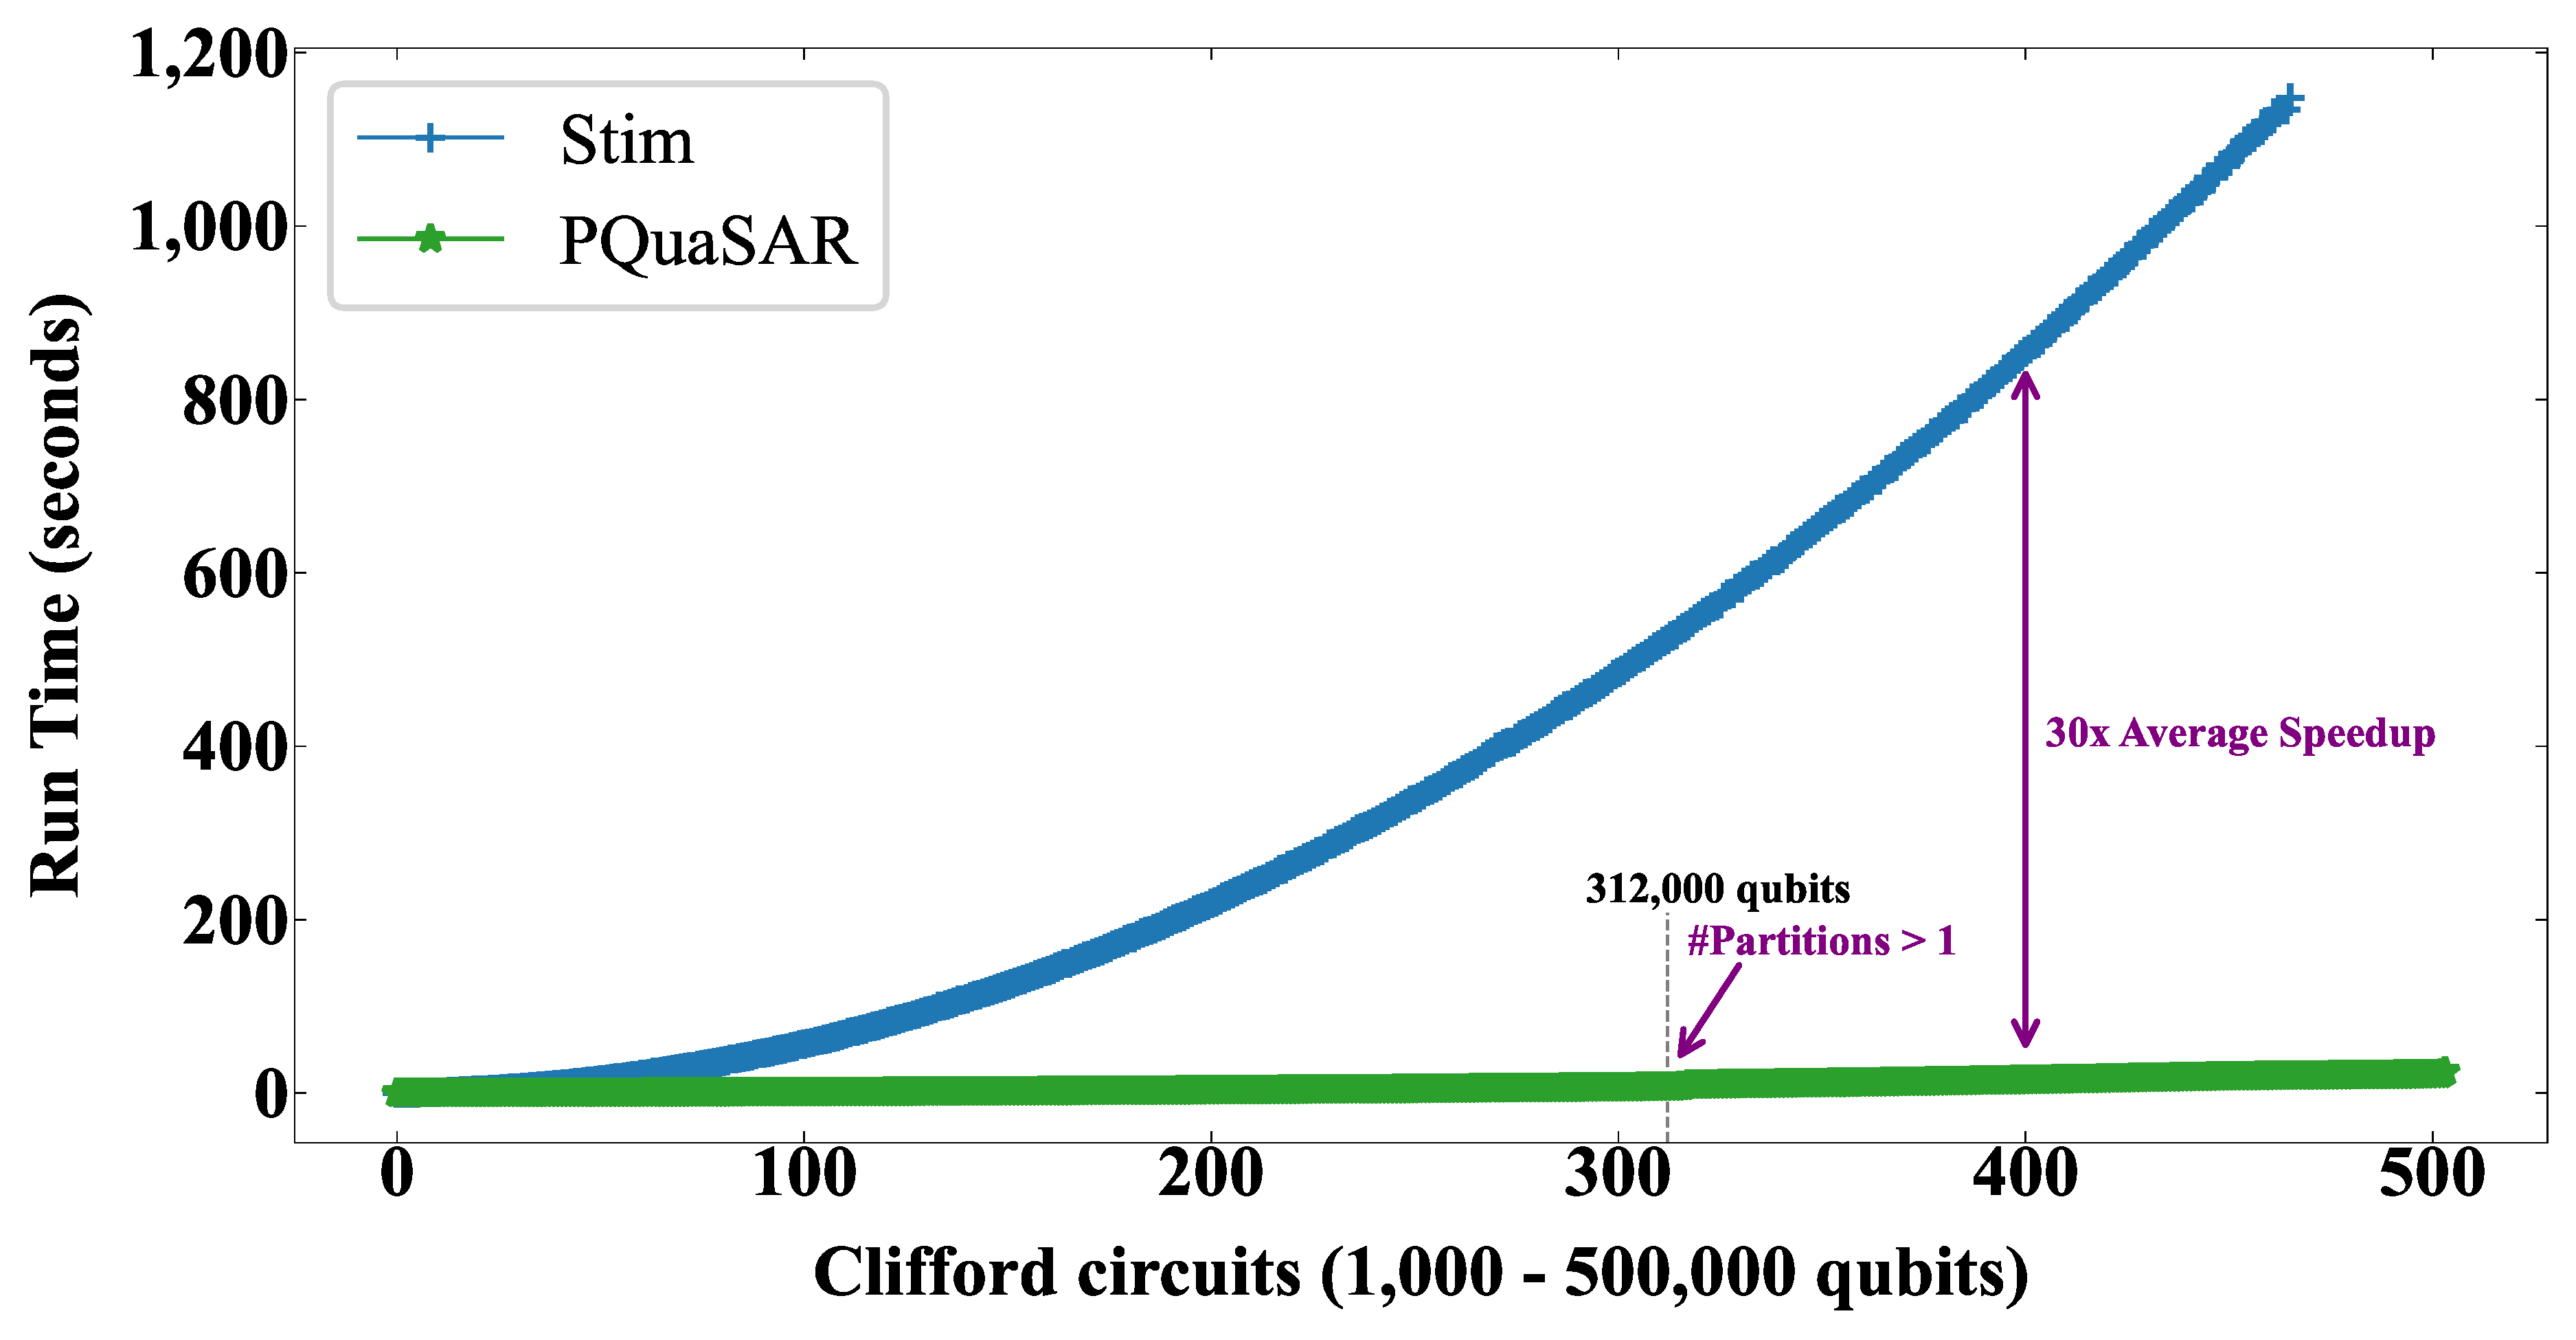
\includegraphics[width=\linewidth]{time_cactus.pdf}
		}
		\quad
		\subfloat[]{
			\label{fig:energy}
			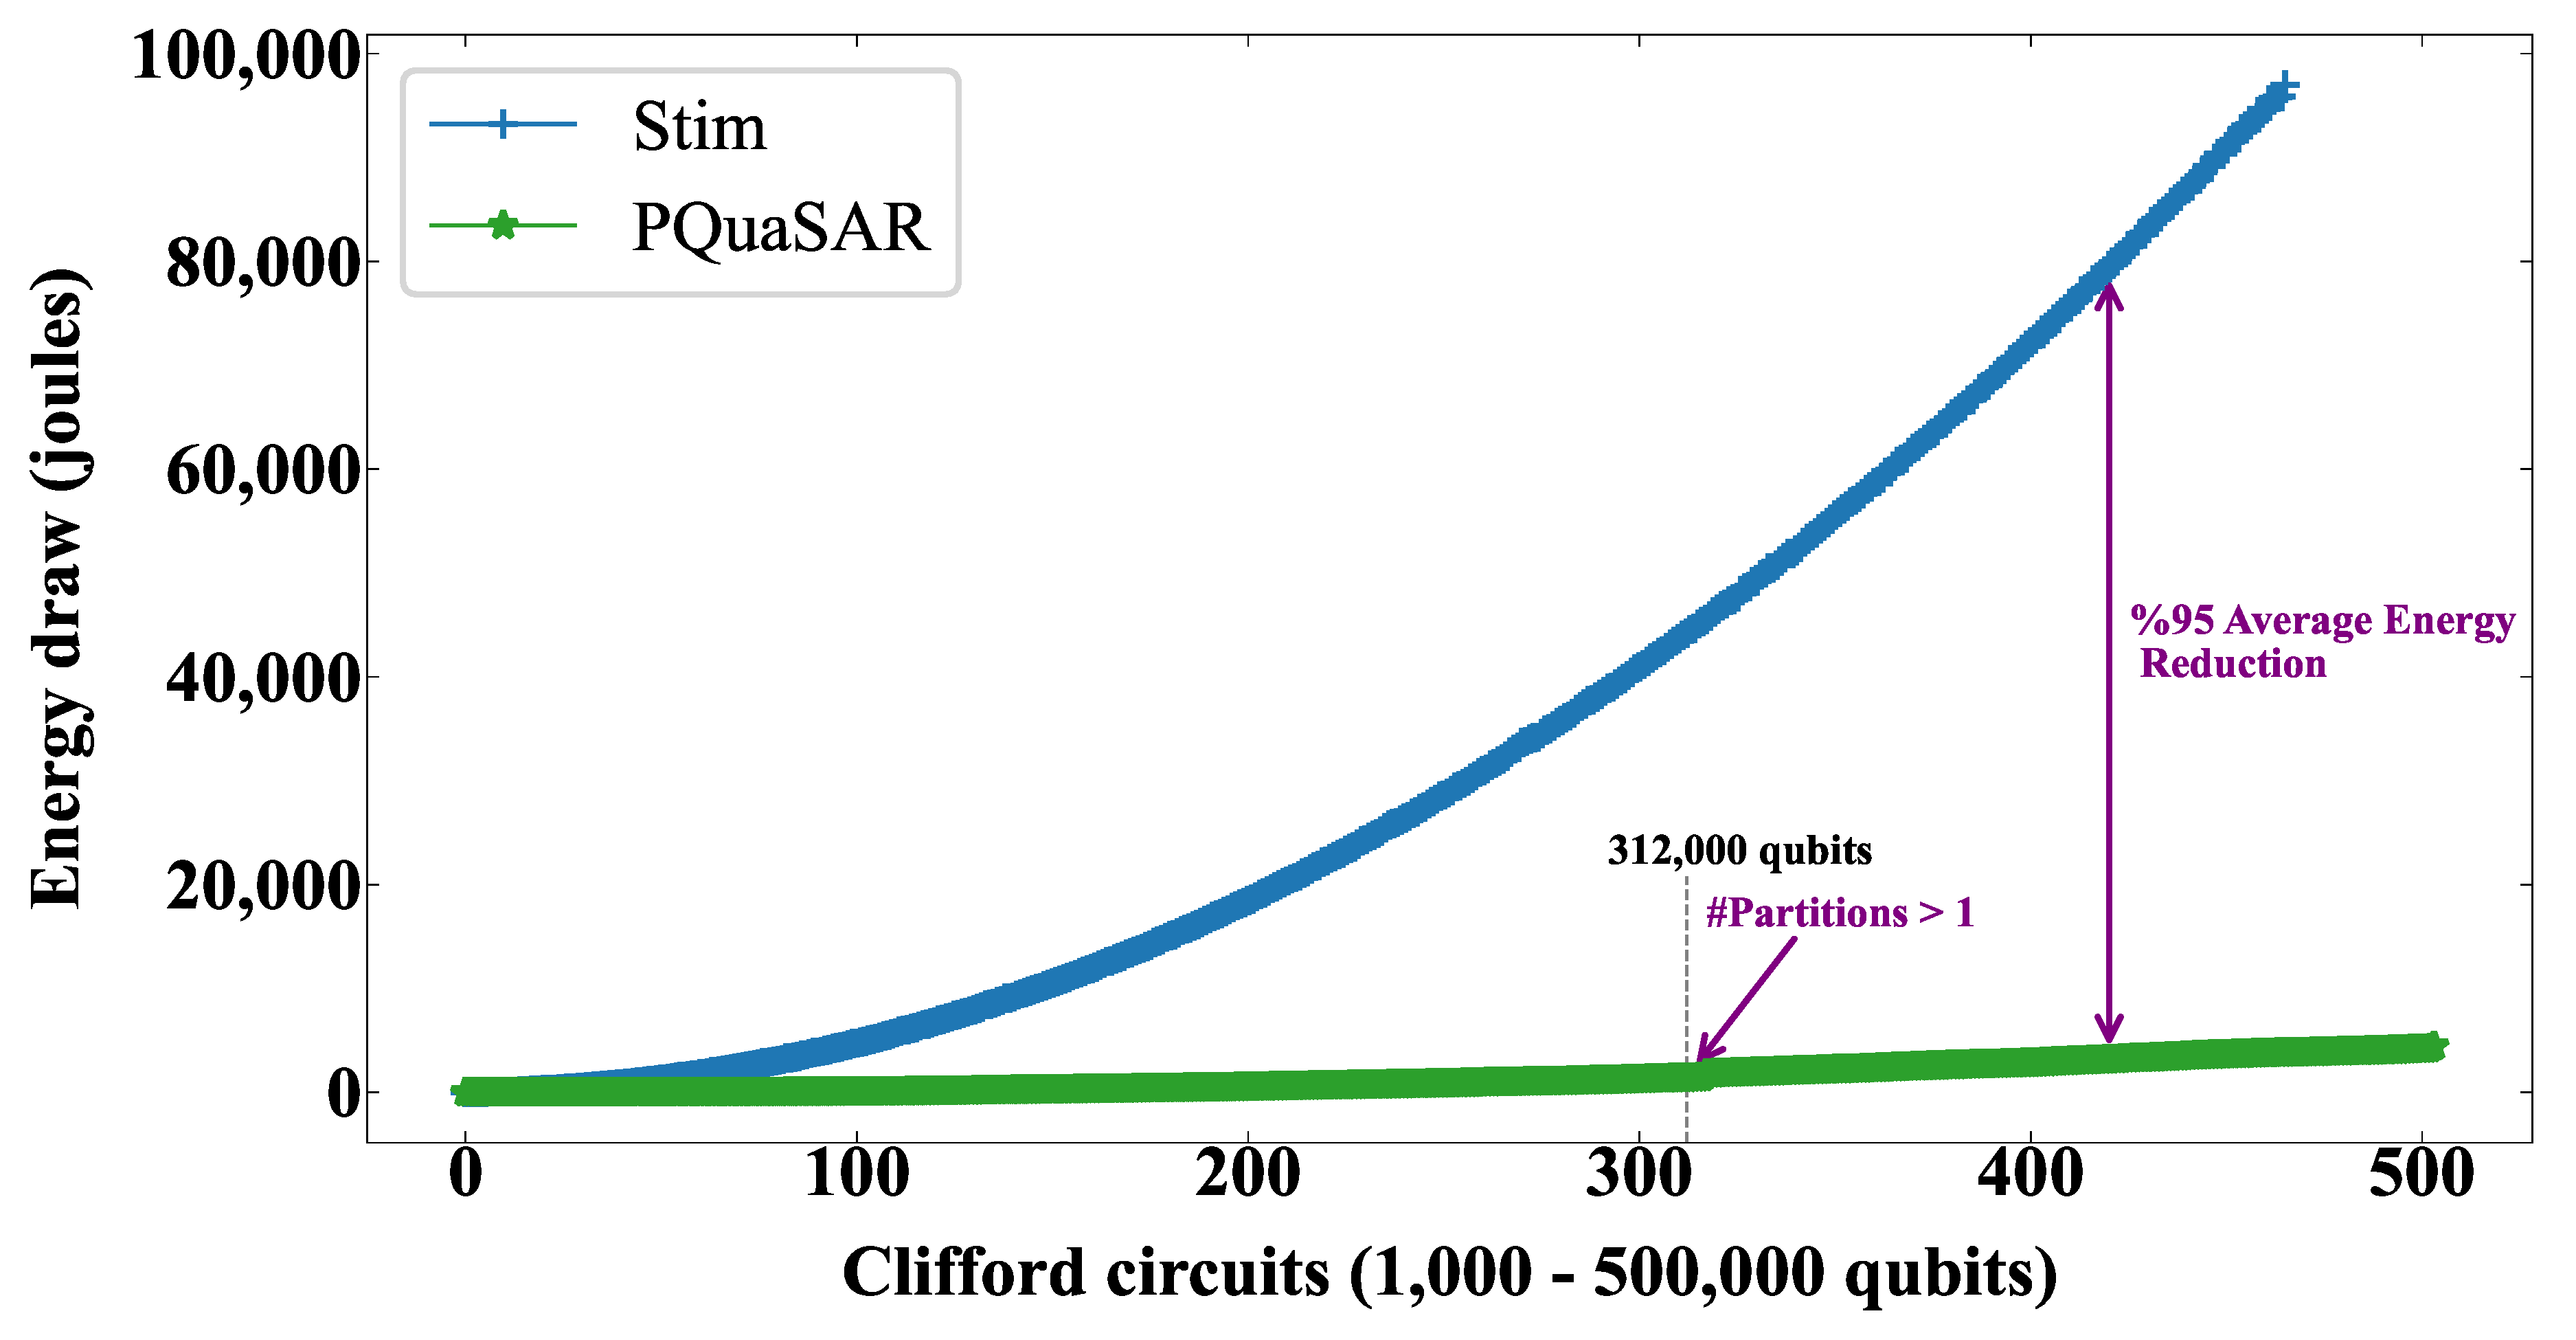
\includegraphics[width=\linewidth]{energy_cactus.pdf}
		} 
	}
	\caption{Simulation performance.}
	\label{fig:performance}
\end{figure*}

\begin{table}[htp]
	\scriptsize
	\renewcommand{\arraystretch}{1.2}
	\setlength{\tabcolsep}{2.9pt}
	\caption{Statistics for a selection of ten circuits (qubits in thousands).}
	\label{tab:quasarq}
	\centering
	\adjustbox{max width=1\linewidth} {
		\begin{tabular}{lrrrrrrrr}
    \hline\hline
    \textbf{Qubits} & \textbf{Initial} & \textbf{Schedule} & \textbf{Simulation} & \textbf{Simulation speed} & \textbf{Energy draw} & \textbf{Tableau} & \textbf{Tableau} & \textbf{Circuit} \\
    \bm{$(\times 1000)$} & \textbf{time (s)} & \textbf{time (s)} & \textbf{time (s)} & \textbf{(GB/sec)} & \textbf{(Joules)} & \textbf{partitions} & \textbf{memory (GB)} & \textbf{memory (GB)} \\
    \hline
    50 & 0.09  & 0.06  & 0.37  & 163   & 37    & 1     & 0.6   & 0.05 \\
    100 & 0.18  & 0.11  & 1.46  & 164   & 289   & 1     & 2.39  & 0.1 \\
    150 & 0.3   & 0.17  & 3.31  & 163   & 697   & 1     & 5.37  & 0.14 \\
    200 & 0.43  & 0.22  & 5.95  & 161   & 1247  & 1     & 9.54  & 0.19 \\
    250 & 0.5   & 0.27  & 9.5   & 157   & 2015  & 1     & 14.91 & 0.23 \\
    300 & 0.59  & 0.33  & 13.73 & 157   & 2911  & 1     & 21.46 & 0.28 \\
    350 & 0.7   & 0.39  & 25.06 & 156   & 5144  & 2     & 19.48 & 0.32 \\
    400 & 0.79  & 0.45  & 32.32 & 158   & 6556  & 3     & 16.96 & 0.37 \\
    450 & 0.88  & 0.51  & 40.84 & 158   & 8244  & 3     & 21.46 & 0.41 \\
    500 & 0.97  & 0.56  & 43.88 & 161   & 9045  & 4     & 17.67 & 0.46 \\
    \hline
\end{tabular}%



	}
\end{table}


Figure \ref{fig:time} gives the runtime peformance of both simulators. \quasarq time includes the intial time (memory allocations, parsing, etc.), the scheduling time of Alg.\ref{alg:scheduler} and the simulation time of Alg.\ref{alg:simulator}. As revealed by the plot, \quasarq runtime is almost constant with outstanding speedup of 30$\times$ faster than \stim. At circuit 312 (312,000 qubits of depth 100), \quasarq starts to partition the tableau due to the demanding tableau space. Thus, a tiny step in runtime can be noticed at the former data point.  One remark to mention, as \stim supports measurements, an extra tableau for the destablizers is needed \cite{stim, aaronson2008improved}. Destabilizers are the anti-commutators of stabilizers  \cite{aaronson2008improved}, hence they do not impose any extra calculations beyond the stabilizers operations. In \stim the stabilizer bits are only propagated to the destabilizers tableau to avoid any computational overhead. Therefore, the runtime of stim technically reflects the operations performed by the stabilizers tableau.
Figure \ref{fig:energy} compares the energy consumption in Joules of \quasarq versus \stim. Remarkably, our simulator can save up to \%90 of energy against \stim. This implies that our parallel simulator is not only fast but also more energy-efficient when implemelnted on the GPU.

Table \ref{tab:quasarq} reports some statistics for a selection of ten circuits. Clearly, the initial and scheduling time are negligible w.r.t. the simulation time. the \emph{simulation speed} measures how many bytes in the tableau are processed per second. This gives indication how fast Alg.\ref{alg:simulator} can be on the GPU. For the 50 case, our simulator could achieve a speed of 163 GB/sec.
Regarding tableau allocation, \quasarq, with the new tableau partitioning mechanism, occupies at most 22GB of memory no matter how many qubits are simulated. See \emph{tableau memory} in Table \ref{tab:quasarq} for exact numbers. Even, when \quasarq supports measurements, 24GB would suffice for the extra destabilizers tableau at the expense of more partitions.
On the contrary, \stim consumed up to 256GB until it eventually ran out of memory on circuit 467. This means that \quasarq can save up to \%90 of memory space compared to \stim.



\subsection{Application: Equivalence checking of Clifford circuits}

As a demonstration of our simulator's capabilities, we perform equivalence checking of Clifford circuits (up to global-phase) \todo{was global-phase defined?} using the algorithm from \cite{EC}. (......we do this for such and such circuits.........). 

The task of equivalence checking of quantum circuits is central to the optimization and compilation of circuits as it can be a subroutine of those. For that reason, it is important to be able to perform circuit equivalence as fast as possible. 

\todo[inline]{Some figure with the equivalence checking benchmarks}





\bibliographystyle{splncs04}
\bibliography{lit}	
	
	
\end{document}






